% Template to be used while publishing
% a scientific work (PhD Thesis etc.)
% at the EDOC-Server of HU-Berlin
%    developed 2003-2008 by
% AG Elektronisches Publizieren,
% Computer- und Medienservice,
% Humboldt-Universitaet zu Berlin
%    with friendly support of
% TeX-Stammtisch in Berlin

% $Revision: 19 $
% $HeadURL: svn+ssh://ryckojox@svn.cms.hu-berlin.de/svn/projects/epub/latex/hudiss/mustermann.tex $
% $Date: 2009-07-03 15:49:19 +0200 (ptk, 03 lip 2009) $
% $Author$
% $Id: mustermann.tex 19 2009-07-03 13:49:19Z ryckojox $

% Questions, comments, support:
%    edoc-latex@cms.hu-berlin.de

% Documentation and information about the conditions of a publication:
%    http://edoc.hu-berlin.de/e_autoren/latex

% Upload:
%    https://edoc.hu-berlin.de/cgi/dokupload/dokupload.cgi

\documentclass[openright,% 
chapterprefix=true, appendixprefix=true, %
bibliography=totoc,
listof=totoc,
index=totoc,
fleqn,
BCOR=10mm,
%firstinits=true
]{scrbook}[2007/12/24]

% The following package is necessary.
% To change the default options of the packages, use the key=value interface.
% See the documentation for details.
% If you need to use any special characters or LaTeX-commands 
% within the options, use \hudisssetup{} after loading this package,
% otherwise they will NOT work correctly.
\usepackage[    
    % inputenc=utf8, % default - latin1
    fontset=lmodern, % other possible parameters: lmodern, times, palatino
    % natbib={}, %include to use the natbib-package
    % jurabib={}, %include to use the jurabib-package
    % apacite={}, %include to use the apacite-package  
    hints=false, % set to 'false' for submission
    checktabu=false, % set to 'false' for submission
    draft=false, % set to 'false' for submission
    qserie=false
 ]{hudiss}

\hudisssetup{%
    titlepagefont={\Large\sffamily} % Use to change the titlepage font
}

% Fill out all the metadata here:
\hudissmetadata{%
    authorprefix={MSc.}, % e.g. Dipl.-Inf.
    authorfirstname={Jakob J.}, % first name
    authorsurname={Kolb}, % surname
    %authorsuffix={ }, % e.g. Ph.D.
    %authoradd={geboren am 22. April 1983 in Engelskirchen}, % date and place of birth
    doctitle={Heuristic Decision Making in World Earth Models}, % title of the thesis
    docsubtitle={...}, % subtitle of the thesis
    % docsubject={}, % subject of the thesis (used in the properties of the pdf-document)
    approvala={...}, % approvals: a-e
    approvalb={...},
    approvalc={...},
    % approvald={},
    % approvale={},
    degree={\so{doctor rerum naturalium} \\ (Dr. rer. nat.)}, % e.g. Dr. Rer. Nat.
    subject={Physik}, % e.g. Informatik
    specialization={Theoretische Physik},
    faculty={Mathematisch-Naturwissenschaftlichen Fakult\"at}, % in Dativ/Genitiv! e.g. Mathematisch-Naturwissenschaftlichen Fakult\"at II
    university={der Humboldt-Universit\"at zu Berlin}, % e.g. Humboldt-Universit\"at zu Berlin
    dean={Prof. Dr. Elmar Kulke}, % dean of the faculty
    president={Prof. Dr.-Ing. Dr. Sabine Kunst}, % president of the university
    datesubmitted={...}, % the date of the submission
    dateexam={...}, % the date of your last exam
    keywordsen={...}, % english keywords comma separated
    keywordsde={...} % german keywords comma separated
}

% If you wish to load any further packages, 
% make any own adjustments (e. g. for the package fancyhdr)
% or define any own commands
% put ALL of them in the following file:
%  Import packages
\usepackage{epigraph} 		% Allows to add nice quotations at the beginning of chapters
\usepackage{amsmath}		% mathematische Erweiterung, u.a. fr den align-environment
\usepackage{amsfonts}		% fr mathematische Symbole wie \mathbb{R}
\usepackage{amssymb}
\usepackage{amsthm}
\usepackage{multirow}
\usepackage{enumerate}
%\usepackage{sidecap}
\usepackage[section]{placeins}
\usepackage{booktabs}
\usepackage{lscape}
\usepackage{longtable}
\usepackage{
  empheq, % for boxes around equations
        wrapfig, % for wrapped figures in text
        makecell, % for custom formatting in table cells
        hhline, % for custom hlines in tables
        tablefootnote, %for footnotes in tables
        wrapfig, % for figures wrapped in text
        cleveref % for better references
}
\usepackage{makeidx} 		% Create index
\makeindex

\usepackage{chngcntr}		% Make footnote counting continuous throughout the whole document
\counterwithout{footnote}{chapter}

%\usepackage[a-1b]{pdfx}  % Allow compliance with PDF/A standard
\usepackage[sort&compress]{natbib}

\iffalse
%
%  Define custom citation style including paper numbers
%
\usepackage[style=authoryear,maxcitenames=2,maxbibnames=100,natbib=true]{biblatex}
%\usepackage[backend=bibtex,style=authoryear,maxcitenames=2,maxbibnames=100,natbib=true, url=false]{biblatex}

\newbibmacro*{papernum}{%
  \iffieldundef{usera}{%
  }{%
    \addcomma\space
    \printfield{usera}%
  }%
}

\DeclareFieldFormat{labelyear}{%
  \stripzeros{#1}%
  \iffieldundef{extrayear}{%
    \usebibmacro{papernum}%
  }{%
  }%
}

\DeclareFieldFormat{extrayear}{%
  \iffieldnums{labelyear}
    {\mknumalph{#1}\usebibmacro{papernum}}
    {\mkbibparens{\mknumalph{#1}\usebibmacro{papernum}}}}

\addbibresource{bibliography.bib}
%%%
\fi

% easy column vectors
\newcount\colveccount
\newcommand*\colvec[1]{
        \global\colveccount#1
        \begin{pmatrix}
        \colvecnext
}
\def\colvecnext#1{
        #1
        \global\advance\colveccount-1
        \ifnum\colveccount>0
                \\
                \expandafter\colvecnext
        \else
                \end{pmatrix}
        \fi
}
 
\raggedbottom 				% Change page layout style
\allowdisplaybreaks[2]		% Allow page breaks in "align" environment

% Hurenkinder und Schusterjungen verhindern
\clubpenalty9999
\widowpenalty9999
\displaywidowpenalty9999

\usepackage{microtype}
\usepackage{hfoldsty}
\usepackage{ellipsis}
\usepackage{nicefrac}

%  Settings
\setlength{\epigraphrule}{0pt}				%  Remove epigraph rule
\setlength{\epigraphwidth}{0.50\textwidth}		%  Change epigraph width
\setlength{\mathindent}{0pt}				%  Set indent of equations
\setcounter{tocdepth}{1}					%  Set table of contents depth
\setkomafont{caption}{\sffamily\small}
\setkomafont{captionlabel}{\sffamily\bfseries\small}
\renewcommand*{\partpagestyle}{empty}

%  Definitions
\newtheorem{mydef}{Definition}	[chapter]			%  Define customized theorem environment
\newcommand{\nn}[1]{{\it #1*}}				%  Define customized style for index entries

%  Environments
\newenvironment{mytabular}{%				%  Custom tabular environment with sans-serif font
  \sffamily \small
  \tabular
}{%
  \endtabular
}

%  Set preambles

%  Set index preamble
%\setindexpreamble{All page numbers in \textit{italics} (additionally marked by asterisks *) are references to the definitions of the respective terms. In contrast, evenly typeset page numbers refer to further usage of the expressions.
%\par\bigskip}

%  Citation aliases
%\defcitealias{Donges2012b}{Donges et al., in prep., P1} % PRE
%\defcitealias{Wiedermann2012}{Wiedermann et al., in prep., P2} % EPL
%\defcitealias{Feldhoff2012b}{Feldhoff et al., in prep., P3} % EPL
%\defcitealias{Feldhoff2012a}{Feldhoff et al., subm., P4} % PLA
%\defcitealias{Radebach2012}{Radebach et al., subm., P5} % PRE
%\defcitealias{Zou2011}{Zou et al., in press, P6} % EPL
%\defcitealias{Donner2012}{Donner and Donges, 2012, P7} % Acta Geophysica
%\defcitealias{Donges2012}{Donges et al., 2012, P8} % PRE
%\defcitealias{Heitzig2010}{Heitzig et al., 2012, P9} % EPJ B
%\defcitealias{Donges2011c}{Donges et al., 2011b, P10} % PNAS
%\defcitealias{Donges2011b}{Donges et al., 2011a, P11} % NPG
%\defcitealias{Tominski2011}{Tominski et al., 2011, P12} % Viz Conference, London
%\defcitealias{Donner2011a}{Donner et al., 2011b, P13} % IJBC
%\defcitealias{Donges2011a}{Donges et al., 2011c, P14} % EPJ B
%\defcitealias{Donner2011b}{Donner et al., 2011a, P15} % EPJ B
%\defcitealias{Zou2011b}{Zou et al., 2011, P16} % Complex Systems and Complexity Science
%\defcitealias{Zou2010}{Zou et al., 2010, P17} % Chaos
%\defcitealias{Donner2010a}{Donner et al., 2010b, P18} % PRE(R)
%\defcitealias{Donner2010b}{Donner et al., 2010c, P19} % NJP
%\defcitealias{Marwan2009}{Marwan et al., 2009, P20} % PLA
%\defcitealias{Donges2009b}{Donges et al., 2009b, P21} % EPL
%\defcitealias{Donges2009a}{Donges et al., 2009a, P22} % EPJ ST
%
%\defcitealias{Donner2012b}{Donner and Donges, subm., C1} % NOLTA 2012
%\defcitealias{Marwan2010b}{Marwan et al., 2010a, C2} % NOLTA 2010
%\defcitealias{Donner2010d}{Donner et al., 2010a, C3} % NOLTA 2010


% The order of the parts in the document is only our suggestion,
% you can change it, if you wish.
% Don't put any other text between those commands.
% Do not remove the \*matter macros.
% Use standard macros to include new chapters.

\begin{document}
    \frontmatter
        \maketitle
        \cleardoublepage

\null\vfill\itshape

\begin{flushright}
	
\end{flushright}
\thispagestyle{empty}
\upshape\cleardoublepage


        \selectlanguage{english}

\begin{abstract}
...

\end{abstract}

\cleardoublepage

\selectlanguage{ngerman}
\begin{abstract}
...

\end{abstract}

\cleardoublepage

\selectlanguage{english} % Switch back to English to obtain the corrected heading for table of contents

        \selectlanguage{english}

%\renewcommand{\thechapter}{\hspace{-0.45cm}}
\addcontentsline{toc}{chapter}{List of Publications}
\chapter*{List of Publications}

This dissertation is partly based on the following publications. The identifiers, \textit{e.g.}, P1, given below are cited in the text to highlight passages that are connected to one or more of these papers.

\paragraph{Papers}
\begin{enumerate}[P1]
    \item \bibentry{Kolb2019b}
    \item \bibentry{Mueller-Hansen2017}
    \item \bibentry{Donges2018}
    \item \bibentry{Asano2019}
    \item \bibentry{Kolb2019a}

\end{enumerate}

%\paragraph{Conference proceedings}
%\begin{enumerate}[C1]
%\item ...
%
%\end{enumerate}

        
%\renewcommand{\thechapter}{\hspace{-0.45cm}}
\addcontentsline{toc}{chapter}{Acknowledgements}
\chapter*{Acknowledgements}
\begin{minipage}[t][0pt]{\linewidth}

Many individuals and organizations enabled and supported me in writing this thesis.\\

 First of all, I thank Prof. J\"{u}rgen Kurths for the continuous trust and support during the last four years and for hosting me at the Potsdam Institute for Climate Impact Research (PIK). Special thanks go to Jobst Heitzig for day-to-day supervision, for numerous discussions, for plenty of freedom when I needed it and for guidance and holding me accountable when I wanted it.
 I want to thank Ricarda Winkelmann and Jean-Denis Mathias for their willingness to critically evaluate this thesis.
 Many thanks to my colleagues and Friends especially Jonathan Donges, Reik Donner, Marc Wiedermann, Wolfram Barfuss and Benjamin Maier, I much appreciated your extensive comments and feedback on my work in various stages. I want to thank them and all of my other colleagues at the COPAN flagship project also for their input and shared experiences in scientific life and work over the last four years.
 Also, I am deeply indebted to my coauthors, especially Finn M\"{u}ller-Hansen, and Doyne Farmer from whom I have learned a great deal about the strengths and weaknesses of economic models, Yuki Asano, who is one of the most industrious persons that I have met in my life and who constantly pushed us to do better, faster and Maurits Ertsen with whom, during long calls on the phone, I had the most interesting discussions on the meaning of modelling and its limits as an ontological tool.\\


 I am much obliged to the Foundation of German Industries (SDW) for placing their trust in me in the early phase of this project. Their scholarship was so much more than just financial support. I also want to thank the Princeton-Humboldt Cooperation and Collective Cognition Network (CoCCoN), and there within especially Pawel Romanczuk, for the opportunity to participate and providing the funds to repeatedly visit Princeton University.
 I am also grateful for all of those who provided me with library and technical infrastructure especially the European Regional Development Fund (ERDF), the German Federal Ministry of Education and Research and the Land Brandenburg for enabling my work by providing resources on the high performance computer systems at PIK.\\

 I am vary grateful to Winnie Poel for many things but at this point especially for her continued support and the big parts of our shared reproductive labor that she took on during the final stages of writing this thesis.
And last but not least, I feel blessed for my two wonderful daughters who came into my life during the work on this thesis and who never get tired of reminding me that there is plenty of life outside of research.
\end{minipage}

        \tableofcontents
        \listoffigures
        \listoftables
    \mainmatter
        %\renewcommand{\thechapter}{\hspace{-0.45cm}}
\addcontentsline{toc}{chapter}{List of frequently used mathematical symbols}
\chapter*{List of frequently used mathematical symbols}

\begin{tabular}{ll}
...

\end{tabular}

        \selectlanguage{english}

%\renewcommand{\thechapter}{\hspace{-0.45cm}}
%\addcontentsline{toc}{chapter}{Introduction}
\chapter{Introduction}
\label{chapter:introduction}
\cite{Blanchard1979,Gullberg2008,Kummel1989a,Berend2006,Evans2006a}
\section{...}
\citet{Hiebeler2006,wiedermann2015macro,Menck2013}
\citet{Berend2006}


%        \setpartpreamble{\vspace{1cm} \centering \parbox[l]{9cm}{...}}
%        \part{Theoretical foundations} \label{part:theoretical_foundations}

%        \include{chapter02}
%        \include{chapter03}
%	 \include{chapter04}
        \chapter{Heuristic Decision Making in a Social Economic Model of Fossil Resource Usage}
\section{Model Development} 

Previous studies \cite{Ans2013} suggest that feedback through supply-demand price mechanisms will have only limited impact on fossil fuel companies. This is due to the fact, that only approximately 15 \% of investors invest subject to socially responsible guidelines \cite{SIF2014Report} and that divested holdings are, especially in liquid markets, very likely to quickly find their way to less responsible investors. \\
Also, as long as the physical capital relying on fossil fuels already exists, economic reasoning follows that it will be used as long as variable costs are covered.
Therefore, a general economic shift from dirty to clean technology needs changes in investment in physical capital or a political imperative mandated by a (qualified) majority. Therefore, I consider a model focussing on savings and investment decisions appropriate to investigate the possible dynamics of an economic transition towards fossil resource independent technologies.\\
In the following I propose a preliminary scheme of such a model.

\begin{figure}[t]
	\centering
	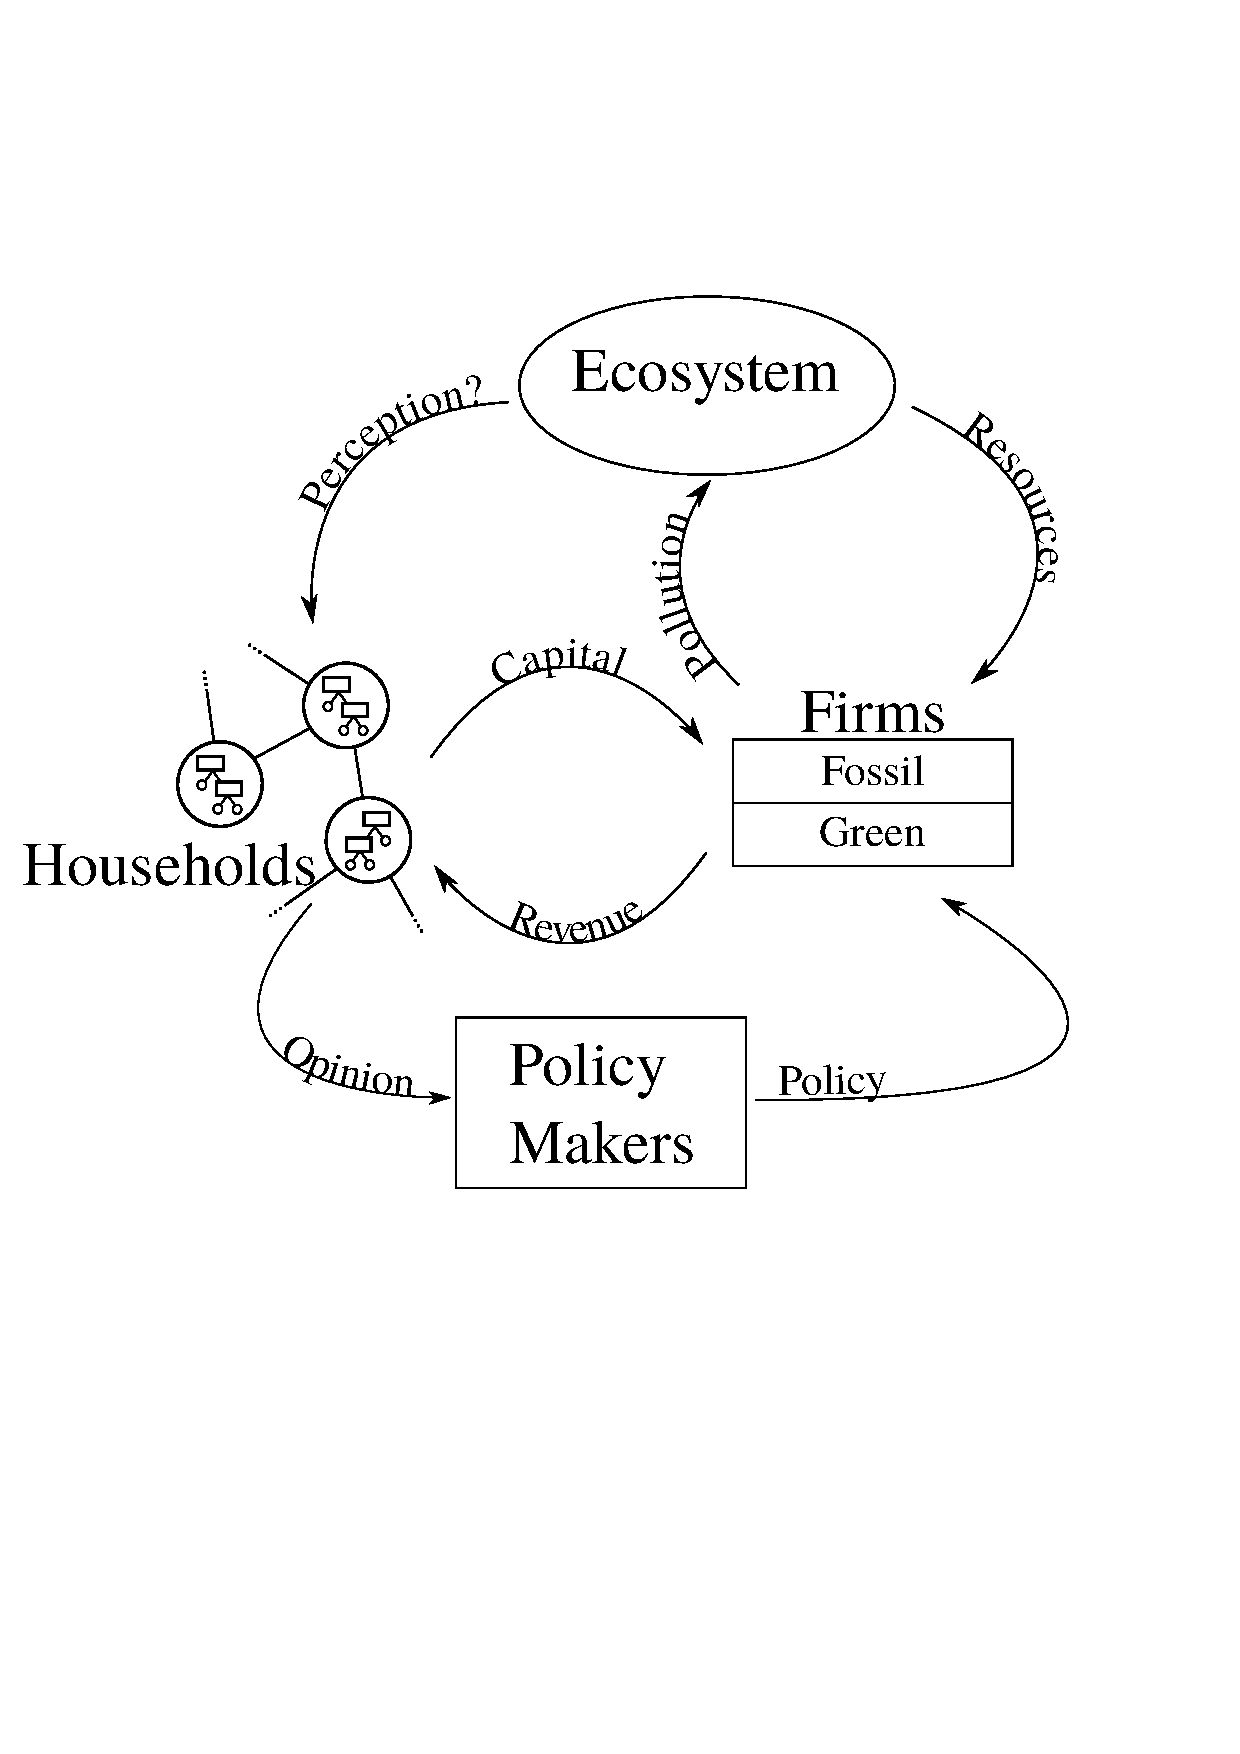
\includegraphics[width =.7 \textwidth]{figures/Model_Scheme.pdf}
	\caption{Schematic sketch of the model including four major components: Households, Firms (grouped by sector), Ecosystem and optional Policy makers.}
	\label{fig:model}
\end{figure}

\subsection{Economic Production}
\label{sec:model_description}

Out model consists of two sectors for production and a set of heterogeneous households that interact via an adaptive complex social network. The production sectors employ different technology. We call them the \textit{clean} and the \textit{dirty} sector for illustrative clarity. The heterogeneous households in the model provide capital $K$ and labor $L$ to both sectors.
In addition, the production technology in the dirty sector depends on the input of an exhaustible (fossil) energy-resource $R$ that is used up in the process. We assume that the technology in the dirty sector is fully developed and adequately described in terms of the total factor productivity. 
Price elasticities of demand for fossil fuel are evidently low in real economies \cite{IMF2011, Hosslinger2017, Labandeira2017}, even with the choice between alternative technologies factored in. We approximate this by setting the elasticity of substitution between the fossil resource and the pair of capital and labor to zero in the dirty sector. This is also in line with contemporary critique of the neoclassical growth models \cite{Daly1997,georgescu1975energy,georgescu1979comments, Ayres2007, Ayres2013} that highlights the generally assumed substitutability of natural resources in production as being physically implausible and lacking empirical evidence.

We acknowledge the common argument for substitutability between capital, labor and energy resources due to a shift in the output of economic production from manufacturing to services and would argue that our model pictures this in a shift of economic production from the dirty sector to the clean one which is described in the following.

The clean sector represents a circular economy in which the output of final goods depends on the machinery, knowledge and effort used in its production and is not limited by entropy laws or resource scarcity on the timescale under consideration. The technology $C$ used in the clean sector is assumed to be still in development and is therefore explicitly modeled.
Following \cite{argote1990learning}, we model technological process as learning by doing according to Wright's law \cite{wright1936factors, Nagy2013} with a one-factor learning curve. We assume that $C$ is proportional to cumulative production but also depreciates with a constant rate $\chi$. Depreciation can be regarded as a human capital effect that leads to knowledge depreciation over time \cite{Kahouli-Brahmi2008}. This is also in line with the empirically observed decrease in learning rates for maturing technologies \cite{argote1990learning}

\begin{equation}
	\dot{C} = Y_c - \chi C.
	\label{eq:learning_by_doing}
\end{equation}

Capital, labor and technology/knowledge are assumed to be mutual substitutes. To satisfy these requirements, we use the following production functions:
\begin{align}
	Y_c &= b_c C^{\gamma} L_c^{\alpha_c}K_c^{\beta_c}, \label{eq:clean_production} \\
	Y_d &= {\mathrm min}\left( b_d L_d^{\alpha_d}K_d^{\beta_d}, e R \right), \label{eq:dirty_production}
\end{align}
Subscripts $c$ and $d$ denote the clean and dirty sector respectively, $L_c$ and $L_d$ are labor shares, $\alpha$ and $\beta$ are elasticities of the respective input factors and $b_c$ and $b_d$ are the total factor productivity and $K_c$ and $K_d$ are the capital stocks for the respective sector. Measuring unit production cost in the number of working hours as in the original study by Wright \cite{wright1936factors}, $\gamma$ is equivalent the elasticity of learning by doing in the clean sector as outlined in \cite{Kahouli-Brahmi2008}.

We assume efficient an usage of resources in the dirty sector, such that
\begin{equation}
    b_d L_d^{\alpha_d}K_d^{\beta_d} = e R
    \label{eq:efficient_dirty_resources}
\end{equation}
where $1/e$ is the resource intensity of the sector. The usage of the fossil resource $R$ depletes a geological resource stock $G$ with the initial stock $G(t=0) = G_0$:
\begin{equation}
    \dot{G} = -R. 
    \label{eq:resource_depletion}
\end{equation} 
In line with the assumptions common in the literature \cite{Dasgupta1974, Perman2003}, the total cost $c_R$ for the usage of the fossil resource depends on the resource use $R$ and the remaining fossil resource stock $G$ such that $\partial c_R / \partial R >0$ and $\partial c_R / \partial G < 0$. We chose the specific form to be
\begin{equation}
	c_R = b_R R^{\rho}\left( \frac{G_0}{G} \right)^{\mu}; \quad \rho \geq 1, \quad \mu > 0,
	\label{eq:resource_cost}
\end{equation}
such that at some point $\partial Y_d / \partial R < \partial c_R / \partial R$ to take into account that some part of the resource is not economic, e.g. its marginal cost exceeds its marginal productivity.
Perfect labor mobility and competition for labor between the two sectors lead to an equilibrium wage $w$ that equals the marginal return for labor:
\begin{equation}
	w = \frac{\partial Y_c}{\partial L_c} = \frac{\partial Y_d}{\partial L_d} - \frac{\partial c_R}{\partial L_d}
	\label{eq:equilibrium_wage}
\end{equation}
with the sum of the labor shares equal to the total amount of labor available:
\begin{equation}
	L_c + L_d = L.
	\label{eq:population}
\end{equation}
We assume physical capital to be specific to the technology employed such that it can only be used in the sector that it has been invested in originally, resulting in separate capital markets for the two sectors. We assume these capital markets to be fully competitive resulting in capital rents equal to marginal productivity:
\begin{align}
	r_c &= \frac{\partial Y_c}{\partial K_c} \label{eq:clean_capital_rent}\\
	r_d &= \frac{\partial Y_d}{\partial K_d} - \frac{\partial c_R}{\partial K_d} \label{eq:dirty_capital_rent}
\end{align}

\subsection{Investment Decision Making}
We model households as bounded rational decision makers \cite{simon1972theories, simon1982models, gigerenzer2002bounded}.
That is, households take their investment decisions, i.e. whether to invest their savings in the clean or the dirty sector, not by forming rational expectations \cite{Evans2006, Kirman2014} but by A) using \emph{heuristic decision strategies} to make robust decisions with sparce information and with limited computational work and B) engaging in \emph{social learning} \cite{bandura1977} to obtain successful decision strategies \cite{Traulsen2010} with reasonable effort.

% Why use Fast and Frugal heuristics for decision making?
Regarding individual decision making, there is ample evidence that real investors rather use a diverse set of heuristic strategies to make investment decisions \cite{Gigerenzer2018} and researchers in the field strongly suggest to consider these so called \emph{Fast and Frugal heuristic} decision models as a complementary alternative to established probabilistic and optimizing decision models. 
In general, Fast and Frugal Heuristics are described in terms of three building blocks; one for information search, one for stopping information search and one for evaluating the available information and drawing a conclusion from it.
We use a decision heuristic called \emph{Take The Best} that is observed to be frequently used in situations where individuals need to decide between one of two options that are comparable in different aspects [CITE]. 
Take the Best has the following building blocks: 1) Search through cues in a predefined order, 2) stop as soon as one cue discriminates between the two options, 3) chose the option with the preferable value on the discriminating cue. \\
This requires a so called \textit{cue order} e.g.\ a hierarchy of validity for the pieces of information that are considered relevant for the decision. \\

% How these heuristics can be interpreted in this context.
Research on perception and decision making in psychology where the concept of Fast and Frugal heuristics was developed usually considers inferential decisions (since they have true and false outcomes and can therefore be benchmarked and evaluated statistically).\\
Nevertheless, Heuristic decision making is a reasonable tool for preferential decisions as well. Although in this context the interpretation of cue orders would be different - namely, they would rather be considered as norms or underlying preferences that apply to the context of the decision. \\
The case of savings decisions that is considered in this model poses an intermediate case between preferential and inferential decisions for a number of reasons. First, there is no immediate feedback on savings decisions, since the return on investment depends on the future development of the economic system which again depends on the savings decisions of all other households and second, we assume that households do not only consider financial but also moral grounds for their savings decisions.
Additionally, I argue that imitation of peers is not only an efficient learning strategy in many situations but also a value in its own - especially if the question is to some extend ethical. 

% Heuristics can be learned from others. This is why we model social learning.
Nevertheless, some strategies are suspected to have more profitable long term results then others as the performance of this decision heuristic depends on the order of the sequence of cues [CITE]. Empirical evidence shows that if participants in an experiment are allowed to share information about their cue orders and respective performance, they do so and thereby greatly increase the speed of learning of cue orders that fit their decision environment compared to individual trial and error reinforcement learning [CITE]. Therefore, we use social learning among households to determine the particular cue order that determines their investment decision making.

% As the outcomes of social learning depend on network topology, we model topology endogenously.
As the outcomes of social learning crucially depend on the structural properties of the complex network of social ties amongst the households \cite{Barkoczi2016}, we model the adaptive formation of this social network endogenously.
A well established principle for the emergence of structured ties in social networks is homophily, i.e. the tendency that similar individuals are linked \cite{McPherson2007, Centola2007, Centola2011}. Especially the concept of value homophily \cite{McPherson2007} is in line with the interpretation of cue orders above not only as a means to the end of making profitable investment decisions but also as an expression of identity and beliefs with regards to clean technology.
The following model specification uses social learning in combination with endogenous network adaptation based on homophily to model the changes in heuristic decision strategies that households use to make investment decisions.

% How I do this technically (Individual Household earnings and investment)
We model $N$ heterogeneous households denoted with the index $i$ as owners of one unit of labor $L^{(i)} = L/N$ and capital $K_c^{(i)}$ and $K_d^{(i)}$ in the clean and dirty economic sector respectively.
Households generate an income $I^{(i)}$ from their labor and capital income which they use for consumption $F^{(i)}$ and savings $I^{(i)}$:
\begin{align}
	I^{(i)} &= w L^{(i)} + r_c K_c^{(i)} + r_d K_d^{(i)}, \label{eq:household_income} \\
	F^{(i)} &= (1-s) I^{(i)}, \label{eq:consumption} \\
	S^{(i)} &= s I^{(i)}. \label{eq:savings}
\end{align}
A binary decision parameter $o_i \in [c,d]$ denotes the sector in which the households decide to invest. As motivated above, we model decision making that is driven by three processes: Heuristic decision making via the Take The Best heuristic, social learning via the imitation of successful cue orders and homophily towards individuals exhibiting the same beliefs as represented by its cue order. \par

% How I do this technically (Heuristic and cue order here)
Concerning the information that households use to make their investment decisions, they are assumed to have no knowledge of the future, e.g.\ they make decisions based solely upon information about the past and present. Possible sources of information are economic indicators such as capital rents in both sectors $r_c$ and $r_d$ and their trends $\dot{r}_c$ and $\dot{r}_d$ as well as observable behavior of other households that they are connected to via the social network and subjective beliefs of superiority of one over the other sector that are not explained by other factors.\\
Each household is characterized by a cue order $O$ containing some or all of the above cues in a specific order. At each time, it uses the Take the Best Heuristic with this cue order to evaluate the information that is available and make an investment decision accordingly.
\par

% How I do this technically (social learning of cue orders)
We describe households as the nodes in a graph of acquaintance relations. Households get active at a constant rate $1/\tau$. When a household $i$ becomes active, it interacts with one of its acquaintances $j$ chosen at random. If they follow the same strategy, i.e. they share the same cue order $O$, nothing happens. If they follow a different strategy, i.e. they differ in their cue order, one of two actions can happen:
\begin{itemize}
	\item Homophilic network adaptation: with probability $\varphi$, the households end their relation and household $i$ connects to another household $k$, that has the same cue order. 
	\item Imitation: with probability $1-\varphi$, household $i$ engages in social learning i.e. it imitates the cue order of household $j$ with a probability $p_{ji}$ that increases with their difference in income.
\end{itemize}
We follow previous results on human strategy updating in repeated interactions \cite{Traulsen2010}, when we assume the imitation probability as a monotonously increasing function of the relative difference in consumption between both households:
\begin{equation}
	p_{ji} =  \left(1 + \exp \left(- \frac{a(F^{(i)} - F^{(j)})}{F^{(i)} + F^{(j)}} \right) \right)^{-1}.
    \label{eq:imitation_probability}
\end{equation}
As opposed to the absolute difference in the original study \cite{Traulsen2010}, the probability in our model depends on relative differences. This dependence on relative differences in per household quantities is crucial for approximation methods as we will discuss later at the end of \ref{sec:large_system_limit}.
We set $a = 8$ to conform to their empirical evidence.
We model strategy exploration as a fraction $\varepsilon$ of events that are random, e.g. rewiring to a random other household or randomly choosing one of the possible cue orders with equal probability.

% Yes, we know, this is only one of the many possible ways to implement such a model.
We acknowledge the fact that different model specifications are possible and interesting.
For instance, we only consider fixed savings rates and the decision between two capital assets and leave the investigation of households setting their savings rates individually to another study \cite{Asano2018}.
Also, this framework might as well be used to test other strategies for decision making such as tallying or pure social learning similar to the approach taken by Barkoczi \cite{Barkoczi2013a}, \cite{Barkoczi2016}

% Capital accumulation of individual households given the model assumptions above.
Given the savings decisions of the individual households, and assuming equal capital depreciation rates $\kappa$ in both sectors, the time development of their capital holdings is given by
\begin{align}
  \dot{K}_c^{(i)} =& \delta_{o_ic} \left( r_c K_c^{(i)} + r_d K_d^{(i)} + w L_i \right) - \kappa K_c^{(i)}, \label{eq:clean_investment}\\
  \dot{K}_d^{(i)} =& \delta_{o_id} \left( r_c K_c^{(i)} + r_d K_d^{(i)} + w L_i \right) - \kappa K_d^{(i)}, \label{eq:dirty_investment}
\end{align}

where $\delta_{ij}$ is the Kronecker Delta. The total capital stocks in the two sectors are made up of the sum of the individual capital stocks as
\begin{equation}
K_j = \sum_i^N K_j^{(i)} = N k_j,
\end{equation}
where $k_j$ is the average per household capital stock of a given capital type.

\subsection{Policy Makers}
\textit{Optional:} \\
Policy makers can implement some carbon tax or carbon cap on economy to incentivize green development. The implementation of such measure depends on the prevalence of opinions amongst voters (are investors a representative sample of voters?) and might be appropriately implemented by a Poisson distributed random variable.

% This is the model. Now lets see what it does.
With the model specifications from above, the parametrization in Tab.~\ref{tab:Parameter_list} and appropriate initial conditions for the dynamic variables, the model can be numerically simulated.
For this, we implemented the dynamics in the multi-purpose programming language python. The implementation of the agent based model, as well as the numerical analysis using the approximation methods described in the following are available on github in \cite{kolb2018}.
In the following, I discuss the technical details ans specification of this implementation.


\begin{table}[t]
	\centering
	\begin{tabular}{r|l}
		Variable & Description \\\hline
		$K^{(i)}_c(t)$ & clean capital of household $i$ \\
		$K^{(i)}_d(t)$ & dirty capital of household $i$ \\
		$G(t)$ & Geological carbon stock \\
                $C(t)$ & Knowledge stock in the clean sector \\
		$O_i(t)$ & opinion/cue order of household $i$ \\
		$o_i(t) \in [c,d]$ & investment decision of household $i$ 
	\end{tabular}
	\caption{Variables of the model with description.}
	\label{tab:independent_variables}
\end{table}

\begin{table}[t]
	\centering
	\begin{tabular}{r|l}
		Variable & Description \\\hline
		$w(t)$   & Wage rate, \\
		$r_j(t)$ & Capital return rate in sector $j$, \\
		$c_R(t)$ & Fossil resource extraction cost, \\
		$Y_j(t)$ & Output of sector, $j$ \\
		$L_j(t)$ & total labor employed in sector $j$, \\
		$K_j(t)$ & Total capital employed in sector $j$, \\
		$R(t)$ & Rate of resource uptake of dirty sector. \\
	\end{tabular}
	\caption{Variables of the model with description.}
	\label{tab:derived_variables}
 \end{table}

 
\section{Implementation} 



\subsection{Solution for Algebraic Constraints: Calculation of wages, resource uptake and capital rent}
\label{sec:algebraic_constraints}

The conditions for labor shares and wages as well as optimal resource uptake pose algebraic constraints for the system of ordinary differential equations that describe the dynamics of the capital stocks $\dot{K}_i^{(j)}$, the resource stock $\dot{G}$ and the dynamics of the knowledge stock in the clean sector $\dot{C}$. In order to solve these differential equations more efficiently, one can solve these algebraic constraints analytically.

To calculate the labor shares $L_c$ and $L_d$ as well as the wages in the two sectors, we use equations \eqref{eq:resource_cost} and \eqref{eq:equilibrium_wage} and for simplicity assume $\rho=1$ and $\mu=2$. We also assume equal labor elasticities in both sectors $\alpha_d = \alpha_c = \alpha$ resulting in
\begin{align}
	w &= \frac{\partial Y_d}{\partial L_d} - \frac{\partial c_R}{\partial L_d} \nonumber \\
	&= \frac{\partial Y_d}{\partial L_d} - \frac{\partial c_R}{\partial R} \frac{\partial R}{\partial L_d} \nonumber = \frac{\partial Y_d}{\partial L_d} - \frac{\partial c_R}{\partial R} \frac{\partial}{\partial L_d} \frac{Y_d}{e} \nonumber \\
	&= \frac{\partial Y_d}{\partial L_d} - b_R\frac{G_0^2}{G^2} \frac{\partial}{\partial L_d} \frac{Y_d}{e} = b_d \alpha L_d^{\alpha-1} K_d^{\beta_d}\left( 1-\frac{b_R}{e}\frac{G_0^2}{G^2} \right)
	\label{eq:dirty_wages}
\end{align}
for the dirty sector and
\begin{equation}
	w = b_c \alpha L_c^{\alpha-1} K_c^{\beta_c} C^{\gamma}
	\label{eq:clean_wages}
\end{equation}
for the clean sector. Combining these results via equation \eqref{eq:population} results in
\begin{equation}
	L = \left( \frac{w}{\alpha} \right)^{\frac{1}{\alpha-1}}\left( \left( b_c K_c^{\beta_c}C^{\gamma} \right)^{\frac{1}{1-\alpha}} + \left( b_d K_d^{\beta_d} \left( 1 - \frac{b_R}{e}\frac{G_0^2}{G^2} \right) \right)^{\frac{1}{1-\alpha}} \right).
\end{equation}
Substituting 
\begin{equation}
	X_c = (b_c K_c^{\beta_c}C^{\gamma})^{\frac{1}{1-\alpha}}, \qquad X_d = (b_d K_d^{\beta_d})^{\frac{1}{1-\alpha}}, \qquad X_R = \left( 1 - \frac{b_R}{e}\frac{G_0^2}{G^2} \right)^{\frac{1}{1-\alpha}}
	\label{eq:substitutions}
\end{equation}
and solving for $w$ yields:
\begin{equation}
	w = \alpha L^{\alpha-1}\left( X_c + X_d X_R \right)^{1-\alpha}.
	\label{eq:wage_result}
\end{equation}
Plugging \eqref{eq:wage_result} into equations \eqref{eq:dirty_wages} and \eqref{eq:clean_wages} results in 
\begin{align}
	L_c &= L \frac{X_c}{X_c + X_d X_R}, \label{eq:clean_labor} \\
	L_d &= L \frac{X_d X_R}{X_c + X_d X_R} \label{eq:dirty_labor}
\end{align}
for the labor shares and plugging this into \eqref{eq:efficient_dirty_resources} results in
\begin{equation}
	R = \frac{b_d}{e}K_d^{\beta_d}L^{\alpha}\left( \frac{X_d X_R}{X_c + X_d X_R} \right)^{\alpha}
	\label{eq:R_result}
\end{equation}
for the use of the fossil resource. Using the results for $L_c$ and $L_d$ together with equations \eqref{eq:clean_capital_rent} and \eqref{eq:dirty_capital_rent}, the return rates on capital result in
\begin{align}
	r_c &= \frac{\beta_c}{K_c}X_c L^{\alpha}\left( X_c + X_d X_R \right)^{-\alpha}, \label{eq:r_c_result}\\
	r_d &= \frac{\beta_d}{K_d}\left(X_d X_R\right) L^{\alpha}\left( X_c + X_d X_R \right)^{-\alpha}. \label{eq:r_d_result}
\end{align}

It is also worth noting that if we assume constant returns to scale with respect to capital and labor, e.g.

\begin{equation}
	\beta_c = \beta_d = 1-\alpha,
	\label{eq:elasticities_restriction}
\end{equation}

(even though it is not necessary for our method) this results in zero profits in both sectors:
\begin{align}
	Y_c &= w L_c + r_c K_c, \nonumber \\
	Y_d &= w L_d + r_d K_d + c_R. \nonumber
\end{align}
To sum up, we solved the algebraic constraints to the ordinary differential equations describing the economic production process resulting in the following equations:
\begin{subequations}
\begin{empheq}[box={\fboxsep=10pt\fbox}]{gather}
	X_c = (b_c K_c^{\beta_c})^{\frac{1}{1-\alpha}}, \qquad X_d = (b_d K_d^{\beta_d})^{\frac{1}{1-\alpha}}, \qquad X_R = \left( 1 - \frac{b_R}{e}\frac{G_0^2}{G^2} \right)^{\frac{1}{1-\alpha}}, \\
	w = \alpha L^{\alpha-1}\left( X_c + X_d X_R \right)^{1-\alpha}, \\
	r_c = \frac{\beta_c}{K_c}X_c L^{\alpha}\left( X_c + X_d X_R \right)^{-\alpha}, \\
	r_d = \frac{\beta_d}{K_d}X_d X_R L^{\alpha}\left( X_c + X_d X_R \right)^{-\alpha}, \\
	R = \frac{b_d}{e}K_d^{\beta_d}L^{\alpha}\left( \frac{X_d X_R}{X_c + X_d X_R} \right)^{\alpha}, \\
        \dot{K}_i^{(c)} = s \delta(o_i - c) (r_c K_i^{(c)} + r_d K_i^{(d)} + w L_i) - \delta K_i^{(c)}, \label{eq:clean_capital_accumulation}\\
        \dot{K}_i^{(d)} = s \delta(o_i - d) (r_c K_i^{(c)} + r_d K_i^{(d)} + w L_i) - \delta K_i^{(d)}, \label{eq:dirty_capital_accumulation}\\
        \dot{G} = - R, \label{eq:sum_up_resource_depletion}
      \end{empheq}
\end{subequations}



\subsection{Limiting cases and timescales}

To estimate some parameters of the system, we analyze some limiting cases of the system and compare them with real world timescales. Such, we can set reasonable values to some parameters.


\subsubsection{Full clean economy}
\label{sec:full_clean_economy}

\begin{wrapfigure}[16]{o}{.55 \textwidth}
	\vspace{-1.8 cm}
	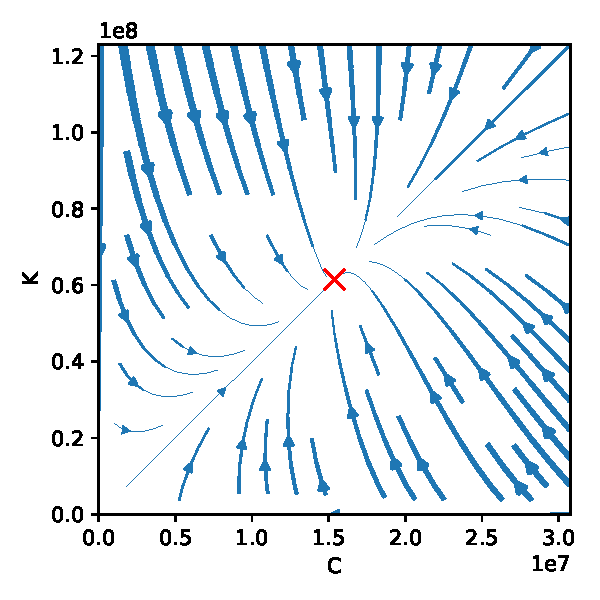
\includegraphics[width = .55 \textwidth]{./figures/phasespace.pdf}
        \caption{Phase space plot of equations \eqref{eq:full_clean_ca1} and \eqref{eq:full_clean_ca2} \label{phase_space_plot}}
\end{wrapfigure}
Along the same lines, we can treat the case of a full clean economy (assuming that the fossil resource is depleted, or the households have for some other reason decided to only invest in clean capital $K_c$). \\
In this case, the equations for capital and knowledge accumulation are
\begin{subequations}
\begin{align}
    \dot{K}_c &= s b_c L^{\alpha} K_c^{\beta} C^\gamma - \delta K_c \label{eq:full_clean_ca1} \\
	\dot{C} &= b_c L^\alpha K_c^\beta C^\gamma - \chi C \label{eq:full_clean_ca2}
\end{align}
\end{subequations}
Assuming that $\alpha + \beta$ = 1, with equal elasticities for capital and labor e.g. $\alpha = \beta$, the stationary points of the system are 
\begin{equation}
  (K_c^*, C^*) = (0,0), \left( \left( \frac{\chi s}{\delta} \right) \left( \frac{s b_c^2 L}{\delta \chi} \right)^{\frac{1}{1-2\gamma}}, \left( \frac{s b_c^2 L}{\delta \chi} \right)^{\frac{1}{1-2 \gamma}}  \right)
	\label{stationary_points}
\end{equation}
where the first one is non hyperbolic and the second one is stable which can be seen in the phase space plot in fig \ref{phase_space_plot} and the corresponding Jacobian
\begin{equation}
	J_{(K_c^*,C^*)} = 
		\begin{pmatrix}
			-\frac{1}{2}\delta & \gamma s \chi \\
			\frac{\delta}{2 s} & \chi \left(\gamma-1 \right)
		\end{pmatrix}
	\label{eq:learning_jacobian}
\end{equation}
whose Eigenvalues are strictly negative:
\begin{equation}
  \lambda_{1,2} = \frac{\delta}{2}(\gamma-1), \quad -\delta.
	\label{eq:learning_eigenvalues}
\end{equation}
The phase space plot in fig. \ref{phase_space_plot} also suggests that there is a trajectory that satisfies 
\begin{equation}
	\frac{K_c(t)}{C(t)} = \frac{K^*_c}{C^*}
\end{equation}
meaning, one has to find a solution to the following ode:
\begin{equation}
	\dot{K}_c = s^{1-\frac{\gamma}{2}} b_c L_c^{\frac{1}{2}}K_c^{\frac{1}{2}(1-\gamma)} - \delta K_c
	\label{eq:learning_trajectory_ode}
\end{equation}
which can be done by means of separation of variables, resulting in
\begin{equation}
  K_c(t) = \left( s^{1-\frac{\gamma}{2}}\frac{b_c L^{\frac{1}{2}}}{\delta} + \exp\left[ (t_0-t) \frac{\delta (1-\gamma)}{2} \right] \right)^{\frac{2}{1-\gamma}}.
	\label{eq:learning_trajectory_solution}
\end{equation}
So, the system approaches its equilibrium approxitely exponentially from below, on a timescale that is given by
\begin{equation}
	t_c^* = \frac{2}{\delta(1-\gamma)}
	\label{eq_learning_equilibrium_timescale}.
\end{equation}
Assuming the same capital depreciation rate for clean capital as for dirty capital previously, together with $\gamma = 1/4$ (as suggested by Jobst Heitzig), the timescale for clean capital accumulation is $t^*_c \approx 53 y$.

\subsubsection{Full on dirty economy}
\label{sec:full_dirty_economy}

Assuming, the fossil resources are very large, the dirty capital stock is significantly more profitable than the clean capital stock and subsequently all households decided to only invest in dirty capital. In this case we can treat the dirty sector isolated:
\begin{equation}
	\dot{K}_d = s I - \delta K_d, \quad I = w L + r_d K_d
	\label{eq:full_dirty_ca1}
\end{equation}
As shown before, $r_d$ is given by:
\begin{align}
	r &= \frac{\partial Y_d}{\partial K_d} - \frac{\partial c_R}{\partial K_d}, \quad c_R = b_R\left( \frac{G_0}{G} \right)^{2} R, \quad Y_d = eR, \\
	&\approx \left( 1-\frac{b_R}{e} \right)\frac{\partial Y_d}{\partial K_d},
	\label{eq:full_dirty_capital_rent}
\end{align}
and similarly for the wage $w$:
\begin{equation}
	w = \left( 1-\frac{b_R}{e} \right)\frac{\partial Y_d}{\partial L}.
	\label{eq:full_dirty_wage}
\end{equation}
So combining these, the income $I$ is equal to
\begin{equation}
	I = \left( 1-\frac{b_R}{e} \right)b_d (\alpha + \beta) L^{\alpha} K_d^{\beta}
	\label{eq_full_dirty_income}
\end{equation}
and using the assumption of zero profits e.g. $\alpha + \beta = 1$ the equation for capital accumulation \eqref{eq:full_dirty_ca1} reads
\begin{equation}
	\dot{K}_d = s\left( 1 - \frac{b_R}{e} \right) b_d L^{\alpha} K_d^{\beta} - \delta K_d
	\label{eq:full_dirty_ca2}
\end{equation}
This ordinary nonlinear differential equation can be solved by separation of variables.
\begin{equation}
  K_d (t) = K_d^{*} \left(1 - e^{(t_0-t)/t_d^{*}} \right)^{\frac{1}{\alpha}}
	\label{eq:dirty_capital_ac_solution}
\end{equation}
where the timescale for capital accumulation $t^*_d$ and the equilibrium dirty capital stock $K^*_d$ are
\begin{equation}
	t_d^{*} = \frac{1}{\alpha \delta}, \qquad K_d^{*} = \left( \frac{s b_d L^\alpha}{\delta}\left(1-\frac{b_R}{e}  \right) \right)^{\frac{1}{\alpha}}.
	\label{eq:full_dirty_capital_equilibrium_values}
\end{equation}
Since the capital depreciation rate $\delta$ is (at least for infrastructure) around 5\% p.a.\ and I assumed $\beta_d=1/2$ for the capital elasticity, the timescale for capital accumulation is $t^*_d \approx 40 y$.
%\newpage




\subsubsection{Fossil resource depletion}
\label{sec:resource_depletion}
\begin{wrapfigure}[16]{o}{.45 \textwidth}
    \vspace{-.8 cm}
    \hspace{-1.8 cm}
	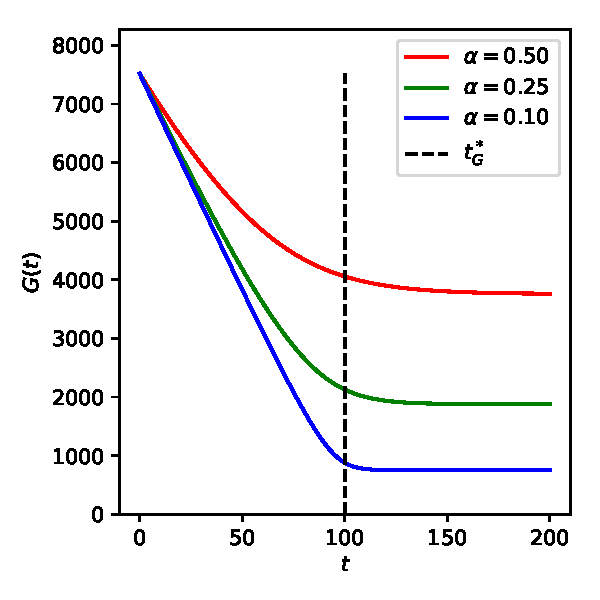
\includegraphics[width = .6 \textwidth]{figures/g_depletion.pdf}
	\caption{Resource depletion in a full dirty economy as described by eq. \eqref{eq:resource_deprec_approx}. The dashed line marks the approximate resource depletion time $t^*_G$. \label{fig:g_depletion}}
\end{wrapfigure}


For this analysis, we assume a full dirty economy like in \ref{sec:full_dirty_economy}. In addition, we assume that we can separate the timescales of resource depletion and dirty capital accumulation, e.g. we assume that dirty capital accumulation happens fast compared to fossil resource depletion such that we can approximate $K_d(t)$ with eq. \ref{eq:full_dirty_capital_equilibrium_values}. Consequently, the ode for fossil resource depletion is given by
\begin{align}
	\dot{G} &= -R \nonumber \\
        &= -\frac{b_d}{e}L^{\alpha}K_d^{*\ \beta_d} \nonumber \\
	&= - \frac{b_d}{e}L^{\alpha}\left(L^{\alpha} \frac{s}{\delta}b_d\left( 1-\frac{b_R}{e}\left( \frac{G_0}{G(t)} \right)^2 \right) \right)^{\frac{\beta_d}{1-\beta_d}}
	\label{eq:resource_deprec_approx}
\end{align}
This means, that unsurprisingly, $G$ converges to a stable fix point $G^* = \sqrt{b_R/e}\ G_0$. Separating variables and substituting $g = G/G_0$ and $\varepsilon = \sqrt{b_R/e}$, the transient dynamic is given by
\begin{equation}
	\int_1^{g(t)} \frac{{\mathrm d} g'}{1 - \varepsilon^2/g'^2} = - \frac{s b_d^2 L}{e \delta G_0} \ t
	\label{eq:resource_transient_integral}
\end{equation}
To get a rough estimate of the time that it takes for the resource to deplete, we assume that $\varepsilon << 1$ and consequently for the most time, $\varepsilon^2/g'^2 << 1$.
This means, that the integrand of the lhs.\ in eq.~\eqref{eq:resource_transient_integral} can be approximated by
\begin{equation}
	\int_1^{g(t)}1+\frac{\varepsilon^2}{g'^2} {\mathrm d}g' = \left[ g' - \frac{\varepsilon^2}{g'} \right]_1^{g(t)} = g(t) - \frac{\varepsilon^2}{g(t)} -1+\varepsilon^2.
	\label{eq:resource_transient_solution}
\end{equation}
This results in the implicit approximate solution:
\begin{equation}
  g(t) - \frac{\varepsilon^2}{g(t)} = 1 -\varepsilon^2 - \frac{s b_d^2 L}{e \delta G_0} \ t.
	\label{eq:resource_transient_solution2}
\end{equation}
According to this approximate solution, $g$ reaches $\alpha$ after a finite time $t^*_G$, which I use as the timescale for resource depletion:
\begin{equation}
	t^*_G = G_0\frac{e \delta}{s L b_d^2}\left( 1-\frac{b_R}{e} \right)
	\label{eq:resource_depletion_time}
\end{equation}
Figure \ref{fig:g_depletion} shows this resource depletion time in comparison to the numerical solution from eq. \ref{eq:resource_deprec_approx} for different values of $\alpha$ to give an impression of the goodness of the approximation.

There are different estimates for the depletion time of fossil resources ranging from approximately 60 years for crude oil to 100 years for gas and 200 years for coal.
So, we assume $t^*_G \approx 100y$. Using this, the initial resource stock $G_0$, the total population, the integrated world BIP (with an assumed growth rate of 2\%p.a.) we could get approximate estimates for $e$ and a relation of $b_d$ to  $b_R$.

% I use 2015 as the base year for my estimates. To estimate $e$ I use World GDP according to the World Bank database CITE ($75.037 \ 10^{12}$ \$) and world primary energy supply according to the BP statistical review of world energy ($13 \ 647$ Mtoe).
% Accordingly, $e$ is estimated at
% \begin{equation}
%   e \approx \frac{75.037 \; 10^{12} \; \$}{13.647 \; 10^9 \; \rm{toe}} = 5.5 \ 10^3 \left[ \frac{\$}{\rm{toe}} \right]
%   \label{ep:estimate_e}
% \end{equation}

\subsection{Parameter Values}

\begin{table}[t]
	\centering
	\begin{tabular}{r|l|c|l}
          \makecell[l]{Symbol} & \makecell[l]{Default \\ Value} & \rotatebox[origin=c]{90}{Variable} & \makecell[l]{Parameter \\ Description} \\\hline
          $b_c$ & 1 & & \multirow{2}{*}{\makecell[l]{total factor productivity (TFP) in \\the clean and dirty sector. \tablefootnote{As TFP is considered somewhat arbitrary even in economic circles as it is critcized for lacking meaningful units of measurement as well as the heterogeneity of factors that are accounted for. Official statistics  avoid measuring levels and instead construct unitless rates of growth.}}} \\ \hhline{---~}
		$b_d$ & 4 & & \\ \hline
                $\alpha_c$ & $1/2$ & & \multirow{3}{*}{\makecell[l]{Labor elasticities in the clean and dirty sector. \\Are assumed to be equal to allow for analytic \\calculation of labor shares between sectors}} \\ \hhline{---~}
                $\alpha_d$ & $1/2$ & & \\
                && & \\ \hline
                $\beta_c$ & $1-\alpha_c$ & & \multirow{3}{*}{\makecell[l]{Capital elasticities in the clean and dirty sector. \\ Are fixed through the assumption of no profits \\that is equivalent to $\alpha_i + \beta_i = 1$.}} \\ \hhline{---~}
                $\beta_d$ & $1-\alpha_d$ & & \\
                && & \\ \hline
                $\gamma$ & $1/8$ & X & Elasticity of knowledge in the clean sector\\ \hline
                $L$ & 1 & & Total labor. \tablefootnote{As TFP is arbitrary, so is labor (as it only scales total output in our case. Therefore, set it to one.}\\ \hline
                $\rho$ & 1 & X & \multirow{2}{*}{\makecell[l]{Exponents of resource usage $R$ and remaining \\resource stock $G$ in the resource extraction costs $c_R$. }} \\ \hhline{---~}
                $\mu$ & 2 & X & \\ \hline
                $b_R$ & & & \multirow{3}{*}{\makecell[l]{Resource uptake efficiency and fossil usage efficiency for \\fossil resource. Together, they define the fraction of fossil \\resources that is not economically viable $G^* = G_0 \left(b_R/e^\rho\right)^{1/\mu}$.}} \\ \hhline{---~}
                $e$ & 1 & & \\
                & & & \\ \hline
                $G_0$ & & & \multirow{2}{*}{\makecell[l]{Initial fossil resource stock. Set according to \eqref{eq:resource_depletion_time} \\ depending on $b_R$, $e$, $b_d$,  $\delta$, $s$ and $L$.}}\\
                & & & \\ \hline
                $s$ & 0.25 & & Savings rate. \tablefootnote{Default value is roughly in line with data for OECD countries.}\\ \hline
                $\delta $ & $0.06$ p.a. & & \multirow{2}{*}{\makecell[l]{Capital depreciation rate. \\ Is assumed to be equal for both sectors}} \\
                &&\\ \hline
                $\chi$ & 0.1 & & Knowledge depreciation rate \tablefootnote{Commonly estimated somewhere between 10\% p.a. and 30\% p.a.}\\ \hline
		$\tau$ & 1 & X & activity rate of households \\ \hline
		$\varphi$ & $1\leq\varphi\leq1$ & X & rewiring probability given an interaction event
	\end{tabular}
	\caption{Parameters of the model with description.}
	\label{tab:Heuristics_Parameter_list}
\end{table}

There are too many parameters in this model to evaluate the qualitative influence of every single one. Therefore, I will discuss some of them shortly here and fix them to constant values for further considerations. \\

\textit{Side note on physical units and dimensions:} It is widely recognized that the use physical dimensions and units in economic modeling leads to inconsistencies and or economically unreasonable results - see e.g. \cite{Barnett2007}. Coincitentally, the overwhelming majority of macroeconomic models does not use dimensional units. From a physicists perspective this seems curious but I will nevertheless adhere to the standard and not use units with parameters and variables in this model. Last but not least to be able to build on said macroeconomic models without running into inconsistencies or producing economically unreasonable results. \\

\textit{Total factor productivities} (TFP) are defining parameters for a Cobb Douglas production function \eqref{eq:clean_production}, They act as a multiplier to set the total output level given a set of input factors such as labor, capital and knowledge and account for all other unaccounted factors in the production process. As such, they are subject to the above critique of lacking meaningful physical units. This is also one of the reasons that if estimated in econometric studies, one usually avoids actual quantities in favour of dimensionless growth rates or values relative to a given base rate like in e.g. \cite{Gal2013, Hooper1997, Bernstein2018}. Therefore, I set the values for TFP in the clean and dirty sector to $b_c=1$ and $b_d=4$ which is arbitrary (and therefore, so is the output of economic production in my model) but makes sure, that the dirty sector is more productive in a scenario with abundant fossil resources $G$ and low clean technology knowledge stock $C$ which is one of the premisses of the model. \\

\textit{Input factor elasticities} are the second defining set of parameters for Cobb Douglas production functions. They measure the responsiveness of output with respect to a change in input factors. Historically, according to \cite{Douglas1976} the values for $\alpha$ range between approximately 0.5 and 0.75. For simplicity, I set $\alpha=1/2$ which however does not limit the generality of the approximate solutions that are developed later in section \ref{sec:Approximation} ff.\\

\textit{Elasticity of knowledge $\gamma$} is also the rate of learning of technology in the clean sector as discussed in \ref{sec:model_description}. This heavily depends on the technology under consideration. Estimates for learning by doing rates approximately range between 10\% and 20\%. I set $\gamma=1/8$ as default and study its influence on qualitative model dynamics.\\

\textit{Total labor $L$} like total factor productivity scales the overall level of economic output in the model. Since this is arbitrary as discussed above, I set it to one (without loss of generality in the approximation methods developed later).\\

\textit{Exponents of resource usage $\rho$ and remaining resource stock $\mu$} are very hard to estimate from data (also, this is not the focus of this thesis). I therefore set them to arbitrary values $\rho=1$ and $\mu=2$ but test different values for comparison.\\

\textit{Resource extraction efficiency $b_R$ and resource usage efficiency $e$} set the share of fossil resources that is not economically viable \eqref{eq:resource_deprec_approx}. Since in the model the fossil resource is accounted for in arbitrary units, I can set $e=1$ without loss of generality and only vary $b_R$ for the analysis of the models dynamics.\\

\textit{The initial fossil resource stock $G_0$} is determined via \eqref{eq:resource_depletion_time} from the value of other parameters by setting the approximate depletion time of the fossil resource.\\

\textit{The savings rate $s$} indicates the fraction of income that households save on average. I use a fixed savings rate for all households that is set to $s=0.25$ which is roughly in line with data for OECD countries\footnote{see https://data.worldbank.org/indicator/NY.GNS.ICTR.ZS}.\\

\textit{The capital depreciation rate $\delta$} is assumed to be equal in both sectors. Capital depreciation rates strongly depend on the type of capital under consideration.\\

\textit{The knowledge depreciation rate $\chi$ in the clean sector} is influenced by different factors. Tacit individual knowledge depreciates with a rate that can be approximated by the rate of workers leaving the workforce. 

\iffalse
\subsubsection{Opinion spreading in the adaptive voter model}
A common way to describe the dynamics of the adaptive voter model in terms of macroscopic variables is the pair approximation.
For simplicity, lets assume a system with two possible opinions $A$ and $B$, on a network with $N$ nodes and $K$ edges.
We describe the model using a vector $(x, y, z)^T$:
\begin{equation}
	x = \frac{[A]-[B]}{N}, \quad y = \frac{[AA]-[BB]}{K}, \quad z = \frac{[AB]}{K}
	\label{avm_variables}
\end{equation}
There are four possible events in the system
\begin{itemize}
	\item 1. an A node rewiring,
	\item 2. a B node rewiring,
	\item 3. an A node adapting a B node and 
	\item 4. a B node adapting an A node.
\end{itemize}
The probabilities for these events to happen are
\begin{align}
	p_1 &= \varphi\frac{z(1+x)}{2(1+y)}, \quad p_2 = \varphi \frac{z (1-x)}{2(1-y)} \\
	p_3 &= (1-\varphi)\frac{z(1+x)}{2(1+y)}1/2({\mathrm tanh}(\Delta I)-1),\\
	p_4 &= (1-\varphi)\frac{z(1-x)}{2(1-y)}1/2({\mathrm tanh}(-\Delta I)-1)
	\label{avm_event_ps}
\end{align}
and their influence on the state vector $s = (x, y, z)^T$ are $s' = s + s_i$ with $s_i$ one of the following:
\begin{align}
	s_1 &= \colvec{3}{0}{1}{-1}, \quad s_3 = \colvec{3}{-2}{-2k\frac{1+y}{1+x}}{-1+2k\frac{1-y-2z}{1-x}-\frac{1-y-2z}{1-y}}\\ 
	s_2 &= \colvec{3}{0}{-1}{-1}, \quad s_4 = \colvec{3}{2}{2k\frac{1+y}{1+x}}{-1+2k\frac{1-y-2z}{1-x}+\frac{1-y-2z}{1-y}}
	\label{avm_event_effects}
\end{align}
Such that in the limit for large N, one gets deterministic equations for $x$, $y$ and $z$:
\begin{align}
	\frac{\dot{x}}{\tau} =& -(1-\varphi)\frac{z}{2}\frac{1-x}{1-y}({\mathrm tanh}(\Delta I)-1) + (1-\varphi)\frac{z}{2}\frac{1+x}{1+y}({\mathrm tanh}(-\Delta I)-1) \\
\frac{\dot{y}}{\tau} =& \quad \varphi\frac{z}{2}\left( \frac{1+x}{1+y} + \frac{1-x}{1-y} \right) + (1-\varphi)kz\left( {\mathrm tanh}(-\Delta I) - {\mathrm tanh}(\Delta I) \right) \\
	\frac{\dot{z}}{\tau} =& -\varphi\frac{z}{2}\left( \frac{1+x}{1+y} + \frac{1-x}{1-y} \right) \nonumber \\
	& + (1-\varphi)\frac{z}{2} \left[ \frac{1+x}{1+y} \frac{1}{2}({\mathrm tanh}(\Delta I)-1) \left( (1+y-2z)\left( \frac{2k}{1+x}-\frac{1}{1+y} \right)-1 \right) \right. \nonumber \\
	& \hspace{1.9 cm} + \left.\frac{1-x}{1-y}\frac{1}{2}({\mathrm tanh}(-\Delta I)-1)\left( (1-y-2z)\left( \frac{2k}{1-x}-\frac{1}{1-y} \right)-1 \right)  \right]
	\label{avm_ode}
\end{align}
assuming that the income difference $\Delta I$ between different cue orders is sufficiently large, this can be reduced to
\begin{align}
	\frac{\dot{x}}{\tau} =& -(1-\varphi)\frac{z}{2}\frac{1-x}{1-y} \\
\frac{\dot{y}}{\tau} =& \quad \varphi\frac{z}{2}\left( \frac{1+x}{1+y} + \frac{1-x}{1-y} \right) + (1-\varphi)kz \\
	\frac{\dot{z}}{\tau} =& -\varphi\frac{z}{2}\left( \frac{1+x}{1+y} + \frac{1-x}{1-y} \right) \nonumber \\
	& + (1-\varphi)\frac{z}{2} \left[ \frac{1+x}{1+y} \left( (1+y-2z)\left( \frac{2k}{1+x}-\frac{1}{1+y} \right)-1 \right) \right]
	\label{avm_ode_reduced}
\end{align}
and from this we see, that the timescale for $x$ to reach its equilibrium values is roughly 
\begin{equation}
	t_a^* = \tau(1-\varphi)
	\label{avm_timescale}
\end{equation}
Since, at least according to my impression, people don't really change their minds or make new friends too often, I propose keeping this timescale between $1<t_a^*<10$ years.
\fi
\subsection{Opinion formation and decision making}
\label{sec:oppinion_formation_and_decision_making}

Households use the Take the Best heuristic to make investment decisions. This heuristic chooses between two options. Therefore, it sequentially evaluates cues (pieces of information), and as soon as one discriminates, it takes the option with the higher value on the discriminating cue. Possible cues in our model are:
\begin{itemize}
	\item[0] investment is dirty,
	\item[1] investment is clean,
	\item[2] Capital return rate $r_c$ and $r_d$,	
	\item[3] trend of capital return rates $\dot{r}_c$ and $\dot{r}_d$, interpolated from previous capital rents,
	\item[4] action observed in the majority of neighbors.
\end{itemize}
Preferences or opinions (I use the expressions synonymously in the context of this model) of the households are combinations of these cues without repetition. Investment decisions according to these preferences are updated immediately. \\
Since the number of possible combinations of these opinions is large ($38$) and consequently, to get statistically valid results one would need a very large number of households ($ ~ 10^2 \times 38$), which would be computationally expensive, we reduce the number of cue combinations to a set of presumably relevant `types':
\begin{itemize}
	\item [[2, 3]]: myopic investor,
	\item [[3, 2]]: trend sensitive investor,
	\item [[4, 2]]: myopic herder,
	\item [[4, 3]]: trend sensitive herder,
	\item [[4, 1]]: Green conformer,
	\item [[4, 0]]: Conservative conformer,
	\item [[1]]: `Gutmensch',
	\item [[0]]: Redneck
\end{itemize}
It is assumed, that these opinions that are the reasoning for individual decision making are spread amongst households in an opinion dynamics process. This opinion dynamics process is a variation of the adaptive voter model. The activity of households is governed by a poison process with mean waiting time $\tau$. If a households becomes active, it randomly chooses one of its neighbors to interact with and if they are of different opinion, there are two possible options:
\begin{itemize}
	\item [1)] with probability $\varphi$ the households cuts the link to its neighbor and connects to a random neighbor with the same opinion,
	\item [2)] with probability $1-\varphi$ they compare their income and with probability $P(x_k \rightarrow x_j)$ the household adopts the opinion of its neighbor.
\end{itemize}
The imitation probability monotonously increases with the income difference between the households: 

\begin{equation} 
	P(x_k \rightarrow x_j) = 1/2 ({\mathrm tanh}(I_k - I_l)-1).
	\label{primitive_imitation_probability}
\end{equation}

To eliminate pathological attractors of this dynamic (as mentioned earlier), a fraction $\varepsilon$ of the rewiring and imitation events are assumed to be random, e.g.\ leading to households making a new connection to another household uniformly at random and in disregard of his opinion or adopting a new opinion amongst the set of opinions that are possible in the system.
\newpage


\section{Results and Discussion}  

To investigate the full dynamics of the model, I conducted different numerical experiments. Since I did not yet find a reliable estimate for $\varepsilon = \sqrt{b_R/e}$, I will conduct experiments for two different values, to point out any qualitative differences, that there might be.

To separate the effects of the adaptive voter dynamic and the heuristic decision making in the model, I conducted separate studies for only the dynamic voter dynamics, only the heuristic decision making and the combination of both effects. \\
Since I am interested in the transition from a dirty to a clean economy, I started the experiment with an equilibrium state with infinite fossil resource supply.\\

\textit{Note that in the first series of experiments, there is no learning yet, e.g. $C \equiv 0$.}

\subsection{Adaptive Voter Experiment}
For the adaptive voter experiment the only possible cues were [0] and [1] such that the only way for changes in investment decisions were imitation of neighbors behavior.
The vertical grey lines show the time at which two thirds of households have opted for investment in the clean sector, assuming that this would be the point when shutting down the dirty sector would be opportune for a policy maker. The background coloring shows the proportion of max.\ economically extractable fossil resources still left in the ground at that point.
\subsubsection{Decisions}
\begin{figure}[t]
	\centering
%	\includegraphics[width = \textwidth]{divestdata/X5o2_Dirty_Clean_Transition_No_TTB/results_N/decisions'alpha'=0o1.pdf}
	\caption{Fraction of households investing in clean capital for $\alpha=0.1$. The vertical grey lines show the time at which two thirds of households have opted for investment in the clean sector, assuming that this would be the point when shutting down the dirty sector would be opportune. }
\end{figure}
\begin{figure}[t]
	\centering
%	\includegraphics[width = \linewidth]{divestdata/X5o2_Dirty_Clean_Transition_No_TTB/results_N/decisions'alpha'=0o05.pdf}
	\caption{Fraction of households investing in clean capital for $\alpha=0.05$. The vertical grey lines show the time at which two thirds of households have opted for investment in the clean sector, assuming that this would be the point when shutting down the dirty sector would be opportune. }

\end{figure}
\subsubsection{Capital Rates}
\begin{figure}[t]
	\centering
%	\includegraphics[width = \linewidth]{divestdata/X5o2_Dirty_Clean_Transition_No_TTB/results_N/capital_rates'alpha'=0o1.pdf}
	\caption{Development of Capital rates for $\alpha=0.1$, $r_c$ is blue, $r_d$ is red. Background color indicates the fraction of economically useful fossil resource that is left in the ground as two thirds of households opt for clean investment.}
	\label{5o2_3}
\end{figure}

\begin{figure}[t]
	\centering
%	\includegraphics[width = \linewidth]{divestdata/X5o2_Dirty_Clean_Transition_No_TTB/results_N/capital_rates'alpha'=0o05.pdf}
	\caption{Development of Capital rates for $\alpha=0.05$, $r_c$ is blue, $r_d$ is red. Background color indicates the fraction of economically useful fossil resource that is left in the ground as two thirds of households opt for clean investment.}
	\label{5o2_4}
\end{figure}
\subsubsection{Market Shares}
\begin{figure}[t]
	\centering
%	\includegraphics[width = \linewidth]{divestdata/X5o2_Dirty_Clean_Transition_No_TTB/results_N/market_shares'alpha'=0o1.pdf}
	\caption{Development of market shares for $\alpha=0.1$}

\end{figure}

\begin{figure}[t]
	\centering
%	\includegraphics[width = \linewidth]{divestdata/X5o2_Dirty_Clean_Transition_No_TTB/results_N/market_shares'alpha'=0o05.pdf}
	\caption{Development of market shares for $\alpha=0.05$}

\end{figure}
Higher alpha apparently leads to earlier transitions from dirty to clean investment.
Comparing figures~\ref{5o2_3} and~\ref{5o2_4} it appears, that higher $\alpha$ leads to higher spikes in the clean capital rent $r_c$ during the transition. This suggest access demand for clean capital that is not supplied by the households. This can be explained by the relative timescales of the resource depletion and opinion spreading resulting in delayed adaptation of opinion prevalence to the changed fitness of the respective opinions.\\
So, apparently, increasing $\alpha$ leads to increasingly abrupt transition with lower fraction of resource remaining in the ground. Also, as expected, higher $\varphi$ leads to slower spreading of successful strategies up to the point where strategies can only be changed through noise/random strategy change. \\
This also shows, that the qualitative signature of the fragmentation transition persists even with noise prevalent in the system.

\subsection{Heuristic Decisions Experiment}

This experiment evaluates the model dynamics for fixed shares of cue orders. There is no rewiring or imitation, just economic dynamics and Heuristic decision making of households according to the cue orders that they have been assigned to in the initial conditions.
Choice of initial conditions for this experiment was somewhat hacky, since 
\begin{itemize}
	\item With cues that take neighbors decisions into account (cue 4 in our example), the clustering in the network of households has considerable influence on the decision making.
	\item I haven't found a way to reproduce the clustering of same opinions that is produced by the adaptive voter model whilst holding the fraction of different opinions constant. 
\end{itemize}
To nevertheless imitate the clustering of similar opinions in the initial conditions, I modified the initial Erd\H{o}s-R\'enyi random graph such that a fraction $\varphi$ of the link in between different opinions were replaced by links between households of equal opinions. 
\par
Figure~\ref{5o3_1} shows that - especially with high shares of cue orders depending on neighbors decisions - increased clustering leads to inhibition of successful investment decision making. Somewhat unsurprisingly, there is some mixtures of cue orders where clean investment decisions are maximal for intermediate clustering of same opinions.
\subsubsection{Decisions}
\begin{figure}[t]
	\centering
%	\includegraphics[width = \linewidth]{divestdata/X5o3_Types_Transition/results_N/decisions'alpha'=0o1.pdf}
	\caption{Fraction of households investing in clean capital for $\alpha=0.1$. The fractions of households with different cue orders investing in either clean or dirty capital are color coded.}
	\label{5o3_1}
\end{figure}
\begin{figure}[t]
	\centering
%	\includegraphics[width = \linewidth]{divestdata/X5o3_Types_Transition/results_N/decisions'alpha'=0o05.pdf}
	\caption{Fraction of households investing in clean capital for $\alpha=0.05$. The fractions of households with different cue orders investing in either clean or dirty capital are color coded.}
	\label{5o3_2}
\end{figure} 
\subsubsection{Capital Rates}
\begin{figure}[t]
	\centering
%	\includegraphics[width = \linewidth]{divestdata/X5o3_Types_Transition/results_N/capital_rates'alpha'=0o1.pdf}
	\caption{Development of Capital rates for $\alpha=0.1$, $r_c$ is blue, $r_d$ is red. Background color indicates the fraction of economically useful fossil resource that is left in the ground as two thirds of households opt for clean investment.}
	\label{5o3_3}
\end{figure}

\begin{figure}[t]
	\centering
%	\includegraphics[width = \linewidth]{divestdata/X5o3_Types_Transition/results_N/capital_rates'alpha'=0o05.pdf}
	\caption{Development of Capital rates for $\alpha=0.05$, $r_c$ is blue, $r_d$ is red. Background color indicates the fraction of economically useful fossil resource that is left in the ground as two thirds of households opt for clean investment.}

\end{figure}
\subsubsection{Market Shares}
\begin{figure}[t]
	\centering
%	\includegraphics[width = \linewidth]{divestdata/X5o3_Types_Transition/results_N/market_shares'alpha'=0o1.pdf}
	\caption{Development of market shares for $\alpha=0.1$, $Y_c$ is blue, $Y_d$ is red.}

\end{figure}

\begin{figure}[t]
	\centering
%	\includegraphics[width = \linewidth]{divestdata/X5o3_Types_Transition/results_N/market_shares'alpha'=0o05.pdf}
	\caption{Development of market shares for $\alpha=0.05$, $Y_c$ is blue, $Y_d$ is red.}

\end{figure}


\subsection{Full Model}
This experiment combines the effects of rewiring and imitation of cue orders and Heuristic decision making of households. Consequently, the decision to invest in clean capital spreads much quicker amongst households. This can be viewed from different angles.
\begin{itemize}
	\item Several cue orders lead to successful investment decisions in both economic regimes. They can be viewed as resilient in a changing fitness landscape.
	\item Cue orders that rely on the investment decision of neighbors tap into the `wisdom of the crowd'. This only works if households with different opinions are sufficiently connected. Otherwise, clusters of households relying on each others decisions stabilize one another (this can be seen for instance in figure~\ref{5o3_1} and~\ref{5o3_2})
\end{itemize}

\begin{figure}[t]
	\centering
%	\includegraphics[width = \linewidth]{divestdata/X5o2_Dirty_Clean_Transition/results_N/decisions'alpha'=0o1.pdf}
	\caption{Fraction of households investing in clean capital for $\alpha=0.1$. The fractions of households with different cue orders investing in either clean or dirty capital are color coded.}
	\label{5o2_1}
\end{figure}
\begin{figure}[t]
	\centering
%	\includegraphics[width = \linewidth]{divestdata/X5o2_Dirty_Clean_Transition/results_N/decisions'alpha'=0o05.pdf}
	\caption{Fraction of households investing in clean capital for $\alpha=0.05$. The fractions of households with different cue orders investing in either clean or dirty capital are color coded.}
	\label{5o2_2}
\end{figure}
\subsubsection{Capital Rates}
\begin{figure}[t]
	\centering
%	\includegraphics[width = \linewidth]{divestdata/X5o2_Dirty_Clean_Transition/results_N/capital_rates'alpha'=0o1.pdf}
	\caption{Development of Capital rates for $\alpha=0.1$, $r_c$ is blue, $r_d$ is red. Background color indicates the fraction of economically useful fossil resource that is left in the ground as two thirds of households opt for clean investment.}

\end{figure}

\begin{figure}[t]
	\centering
%	\includegraphics[width = \linewidth]{divestdata/X5o2_Dirty_Clean_Transition/results_N/capital_rates'alpha'=0o05.pdf}
	\caption{Development of Capital rates for $\alpha=0.05$, $r_c$ is blue, $r_d$ is red. Background color indicates the fraction of economically useful fossil resource that is left in the ground as two thirds of households opt for clean investment.}

\end{figure}
\subsubsection{Market Shares}
\begin{figure}[t]
	\centering
%	\includegraphics[width = \linewidth]{divestdata/X5o2_Dirty_Clean_Transition/results_N/market_shares'alpha'=0o1.pdf}
	\caption{Development of market shares for $\alpha=0.1$, $Y_c$ is blue, $Y_d$ is red.}

\end{figure}

\begin{figure}[t]
	\centering
%	\includegraphics[width = \linewidth]{divestdata/X5o2_Dirty_Clean_Transition/results_N/market_shares'alpha'=0o05.pdf}
	\caption{Development of market shares for $\alpha=0.05$, $Y_c$ is blue, $Y_d$ is red.}

\end{figure}


\section{Conclusion}
\section{Outlook}
Next, I thought I'd implement `campaigners', green investors who are persistent in their opinion and who rewire not preferably to themselves but randomly to households of other opinions. Then I'd experiment on how many of these campaigners are necessary in order to tip the system to a qualified majority of clean investment for a given amount of resource staying in the ground. \\

Learning in the clean sector also seems to be a promising lead. This could result in a number of campaigners and/or explorative investors feeding the clean sector op to a point where it is competitive - making other investors follow their lead.

\subsection{Experiments with learning in the clean sector}

In the next series of experiments, I implemented learning in the clean sector as outlined in section~\ref{eq:learning_by_doing}.
Consequently, with the appropriate choice of parameters, the system becomes bistable with 
\begin{itemize}
	\item one stable state of high fossil resource use, low clean investment and small clean tech.\ knowledge stock,
	\item and one stable state with low fossil resource use, high clean investment and large clean tech.\ knowledge stock.
\end{itemize}
Choice of parameters for the economic system is the following:

\begin{table}[t] 
	\centering
	\begin{tabular}{r|l}
		Parameter & Default Value \\\hline
		$\kappa_c$ & 1/2 \\
		$\kappa_d$ & 1/2 \\
		$\pi$ & 1/2 \\
		$\xi$ & 1/4 \\
		$e$ & 100 \\
		$b_c$ & 0.4 \\
		$b_d$ & 1.2 \\
		$b_R$ & 1 \\
		$s$ & 0.23 \\
		$\delta $ & 0.06 \\
		$P$ & 500 \\
		$G_0$ & $\sim$ 35000 \\
	\end{tabular}
	\caption{Parameter values for numerical studies with learning in arbitrary units.}
	\label{tab:learning_parameter_values}
\end{table}

Choice of parameters for the network amongst households is $N=100$, $p=0.125$ with an Erd\H{o}s-R\'enyi random graph as initial configuration. 

Like before, the initial conditions for the experiment are an equilibrium dirty economy with abundant fossil resources. At the start of the experiment the fossil resource depletion is switched on.\

\begin{figure}[t]
	\centering
%	\includegraphics[width = \linewidth]{divestdata/X5o4_Dirty_Clean_Transition/results_N/decisions'alpha'=0o1.pdf}
	\caption{Fraction of households investing in clean capital with different households types marked by colors. $\alpha=0.1$.}
	\label{fig:learning_decisions0o1}
\end{figure}

\begin{figure}[t]
	\centering
%	\includegraphics[width = \linewidth]{divestdata/X5o4_Dirty_Clean_Transition/results_N/decisions'alpha'=0o05.pdf}
	\caption{Fraction of households investing in clean capital with different households types marked by colors. $\alpha=0.5$.}
	\label{fig:learning_decisions0o05}
\end{figure}
These figures serve well to differentiate between the part of the transition that stems from the decision making and the part that relies on the adaptive voter process.
The plots in the uppermost row of figure~\ref{fig:learning_decisions0o1} and~\ref{fig:learning_decisions0o05} show the effect of only the decision making process (since the adaptive voter dynamic is negligibly slow) in contrast to the plots on the two rows below, that include the effect of the adaptive voter process.\\

But looking at the transition in terms of economic variables, it becomes obvious that it is still mainly driven by the depletion of the fossil resource. This is most visible, if we look at the cost in the dirty sector in figure \ref{fig:learning_dirty_cost0o1} and \ref{fig:learning_dirty_cost0o05}.

\begin{figure}[t]
	\centering
%	\includegraphics[width = \linewidth]{./divestdata/X5o4_Dirty_Clean_Transition/results_N/dirty_costs'alpha'=0o1.pdf}
	\caption{Factor costs in the dirty sector for $\alpha = 0.1$. Solid gray vertical lines indicate the time of qualified majority of clean investment decisions, the transparent gray area marks the standard error of this mean and the dashed/dot dashed gray lines indicate the earliest/latest times of incident. Background colors indicate the fraction of the fossil resource that is still in the ground when the clean majority is reached.}
	\label{fig:learning_dirty_cost0o1}
\end{figure}
\begin{figure}[t]
	\centering
%	\includegraphics[width = \linewidth]{./divestdata/X5o4_Dirty_Clean_Transition/results_N/dirty_costs'alpha'=0o05.pdf}
	\caption{Same as fig.~\ref{fig:learning_dirty_cost0o1} but with $\alpha = 0.05$.}
	\label{fig:learning_dirty_cost0o05}
\end{figure}
On average, this point is reached when the cost of the fossil resource becomes comparable to the cost of other input factors, although there are cases, when this happens  significantly earlier (indicated by the dashed grey line). It would be interesting to look at the exact distribution of these incidents (TO DO).
From the comparison of these figures, it is apparent, that larger alpha (e.g.\ smaller fraction of the fossil resource economically extractable) leads to a larger fraction of the fossil resource remaining in the ground when a clean majority is reached. \textit{note, that this is not in absolute numbers but in relation to the fraction of resource that can be economically extracted}.
This might be due to the fact, that $\alpha$ also influences the difference in return rates from the different kinds of capital resulting in the dirty state of the economy being less `stable' (its basin of attraction becoming smaller and shallower?) such that the system has higher probability to `tip' over into its second (clean) stable state. \\

Maybe interesting to look into: Runs with large amount of fossil resources that are sufficient to sustain a dirty economy for some time, then get scarcer and scarcer until the system tips into the clean state. Look at the distribution of tipping times, maybe use early warning signs (from the fluctuation of clean capital and investment) to predict the probability of tipping depending on the remaining fossil resource.

\subsection{Experiments with a divestment/green investment campaign}
In this experiment, I want to look into the effect that a green investment campaign might have on the transition from a dirty to a clean state of the economic model.\\
The campaign is implemented as follows: In addition to the types of households that were used previously (as described in sec.~\ref{sec:oppinion_formation_and_decision_making}) there is an additional type that I call \textit{campaigner}. Campaigners have the following properties:
\begin{figure}[t]
	\centering
%	\includegraphics[width = \linewidth]{./divestdata/X5o5_Dirty_Clean_Transition/results_N/dirty_costs'alpha'=0o1.pdf}
	\caption{Factor costs in the dirty sector for $\alpha = 0.1$. Solid gray vertical lines indicate the time of qualified majority of clean investment decisions, the transparent gray area marks the standard error of this mean and the dashed/dot dashed gray lines indicate the earliest/latest times of incident. Background colors indicate the fraction of the fossil resource that is still in the ground when the clean majority is reached.}
	\label{fig:campaign_dirty_cost0o1}
\end{figure}
\begin{itemize}
	\item Campaigners persistently invest in clean capital,
	\item Campaigners value their integrity over capital income e.g.\ they do not imitate other households even if they have higher income (in other contexts this behavior is called zealotry),
	\item Other households may become part of the campaign by imitating a campaigner through the established adaptive voter mechanism.
\end{itemize}
\begin{figure}[t]
	\centering
%	\includegraphics[width = \linewidth]{./divestdata/X5o5_Dirty_Clean_Transition/results_N/dirty_costs'alpha'=0o05.pdf}
	\caption{Same as fig.~\ref{fig:campaign_dirty_cost0o1} but with $\alpha = 0.05$.}
	\label{fig:campaign_dirty_cost0o05}
\end{figure}


\begin{wrapfigure}[20]{o}{.55 \textwidth}
	\vspace{-.4 cm}
	%\includegraphics[width = .5 \textwidth]{./figures/remaining_reserves.png}
	\caption{Fraction of economically valuable fossil resources remaining in the ground at the point in time when a qualified clean majority is reached \label{fig:remaining_reserves}}
\end{wrapfigure}

Looking at the costs in the dirty sector again, it is apparent that the initial size of the campaign has significant influence on the transition towards clean investment.This influence is also shown in fig \ref{fig:remaining_reserves}. Although from this plot, no clean tendencies can be deduced except that increasing initial campaign size as well as decreasing rewiring probability both have positive influence on the remaining resources.
Also, with the campaign present, the value of $\alpha$ has larger influence on the resulting fraction of fossil resource staying in the ground. I suspect that this can be explained as follows: As speculated earlier, larger $\alpha$ leads to smaller basin of attraction of the dirty state of the economy. If at a given point in time a fraction of the households is made to invest in the clean sector, this poses a disturbance to the system. This disturbance is more likely to tip the system into its other state, if the barrier between these states is smaller. Additionally, due to learning in the clean sector, a starting investment makes return rates in this sector go up, which leads all households that invest according to trends in return rates to join in - multiplying the effect of the initial investment of the campaigners.\\
Since being a campaigner is an absorbing state in the opinion dynamic, it is clear that eventually all other opinions will vanish. The question is, at what rate this happens and when. Looking at the shares of different types of households in figures \ref{fig:campaign_decisions0o1} and \ref{fig:campaign_decisions0o05} one finds that the fraction of campaigners grows very slowly first and then explodes to leave all other types marginalized.\\
\begin{figure}[t]
	\centering
%	\includegraphics[width = \linewidth]{./divestdata/X5o5_Dirty_Clean_Transition/results_N/decisions'alpha'=0o1.pdf}
	\caption{Household investment decisions marked by household types. Thick red line marks the fraction of households investing in clean capital. The stacked colors below this line mark the fractions these decisions according to the types of household who made them. The stacked colors above the red line indicate the types of households investing in dirty capital. The area in mint green marks the fraction of households that are campaigners.}
	\label{fig:campaign_decisions0o1}
\end{figure}
\begin{figure}[t]
	\centering
%	\includegraphics[width = \linewidth]{./divestdata/X5o5_Dirty_Clean_Transition/results_N/decisions'alpha'=0o05.pdf}
	\caption{Same as fig.~\ref{fig:campaign_decisions0o1} but with $\alpha = 0.05$.}
	\label{fig:campaign_decisions0o05}
\end{figure}



        %% main text
\chapter{Macroscopic Approximation methods for networked agent-based models}
\section{Introduction}
\label{sec:intro}

% Introduction to macroeconomic modeling and the aggregation problem
Macroeconomic models formulate dependencies between aggregate economic variables.
Since Lucas' influential critique, it has become the dominating paradigm that macroeconomic models should built upon microfoundations, i.e., the behavior of individual economic agents \citep{Janssen2016}.
\citet{Lucas1976} argued that using statistical correlations between aggregate variables in models could lead to ineffective policy recommendations because they might not account for changes in agent's decisions as a consequences of introducing a policy.
A historically important example is the observed inverse relation between inflation and employment that can break down if used by policy makers to increase employment.
But with the requirement of microfoundations come several problems in the aggregation of the behavior and decision making of individual agents in the economy.

Two modeling approaches that bridge the gap between microeconomic assumptions and macroeconomic dynamics stand out in the literature: dynamic stochastic general equilibrium (DSGE) modeling, the current workhorse of theoretical macroeconomics, and agent-based modeling (ABMs), a computational simulation approach.
However, both of these approaches have their strengths and limitations regarding the representation of groups of agents and possibilities for model analysis, as we will discuss in the following.

% current state-of-the-art in macroeconomics: DSGE with representative agent(s)
Most DSGE models build on the representative agent approach as a shortcut to circumvent the difficulties arising from the aggregation of heterogeneous and interacting agents.
A representative agent is usually modeled as a utility or profit maximizer.
DSGE models assume that agents have rational expectations when making decisions about the future, i.e., they form fully self-consistent and therefore optimal expectations about the  state of the economy in the future.
Assuming rational expectations implies a strong notion of rationality: agents are assumed to possess and are capable to evaluate all relevant information for their decision problem.
One big advantage of macroeconomic models using the representative agent approach is that they can be solved either analytically or with low numerical effort, allowing for a better understanding of crucial mechanisms in the model than computational simulation approaches do.

% Disadvantages/critique of representative agent
Because the representative agent approach cannot account for interactions within a represented group, models using this approach do not allow for the representation of emergent phenomena.\footnote{We use here a weak notion of emergence, which allows explaining macro-phenomena on the basis of micro-interactions of the systems constituents that differ from the explained macro-phenomena. This is opposed to strong emergence, that embraces the irreducibility of macro-phenomena to lower-level dynamics. For a discussion see \citet{Bedau1997}.}
As \citet{Kirman1992} points out, single-agent utility maximization does not automatically lead to representative agent maximization.
Furthermore, even if a group of agents could be represented by a representative agent, there would be no correspondence between a single agents' preferences and the representative agent's preferences, at least not unless the agents' preferences satisfy very special and unrealistic assumptions (e.g., homotheticity).
The representative-agent approach therefore implies that theoretical macroeconomics reduces macroeconomic phenomena to assumptions about a few different representative agents, leaving out a plethora of explanatory mechanisms for fluctuations in aggregate variables based on intra-group interaction and heterogeneity.
Approaches to represent heterogeneous agents in DSGE models have been used to counter this criticism and add more realism regarding the distribution of agent attributes \citep[see, e.g., the review in ref.][]{Heathcote2009}.
But their solution often require complex numerical methods and cannot integrate local interactions between agents.
% Critique of rational expectations
These problems are strongly related to the assumption of rational expectations.
While in the model, the assumption implies that agents are aware of the constraints and dynamics of the model and take this into account for their decisions. Yet, in the real world, this means that all economic agents know how all mechanisms in the economy work -- a rather strong assumption for many applications.
However, rational expectations are not a prerequisite for adequate microfoundations that pass the Lucas critique \citep{Evans2006}.
For many real-world phenomena, it is therefore more plausible to model agents that adapt their expectations to changing economic circumstances and whose decisions are influenced by social interactions and social context.

% Introduction to agent-based models
ABMs offer a promising framework to model such groups of heterogeneous and interacting agents.
They allow implementing various individual decision models that are behaviorally more realistic than standard economic assumptions. ABMs are then used to study emergent, aggregate phenomena from local interactions \citep{Epstein1999, Tesfatsion2006, Hamill2016}.
These interactions can be structured by spatial embedding of agents or by adaptive social networks \citep{Gross2008,Holme2006a}.
Fluctuations in aggregate variables in ABMs do not only arise from exogenous shocks as in DSGE models but primarily from irregularities in local interactions. Therefore, they offer an avenue for explaining various interesting phenomena studied in empirical macroeconomics.
Furthermore, agent heterogeneity can be modeled as an endogenous result of interactions and not as an effect of predetermined heterogeneity in preferences or asymmetric shocks.

% Disadvantages/critique of agent-based models
However, ABMs are often very detailed so that they can only be simulated numerically. Because the model mechanisms are difficult to trace in the `black box' of a computational model, the results of ABMs are often difficult to interpret and cannot provide mathematically sound proofs of relationships between model variables. There has been some progress in the standardization of model descriptions for ABMs \citep{Grimm2006}, but the lack of standardization, e.g., of decision rules, makes the models difficult to compare \citep[][p. 239]{Hamill2016}. Even though there are various techniques available for comprehensive model analysis \citep{Lee2015}, a systematic model exploration is uncommon and mostly limited to sensitivity analysis of crucial parameters.

% Bringing the two together
Aggregation methods from statistical physics can bridge the gap between analytic macroeconomic models and agent-based computational models \citep[for a review of physics methods in social modeling, see ref.][]{castellano2009statistical}. In contrast to macroeconomic models, these approaches account for local interactions and use aggregation techniques to derive macro dynamics, providing a true microfoundation of the resulting macromodel.
These kinds of approximation methods have found more interest in the fields of financial economics, behavioral finance and evolutionary game theory recently and have produced interesting and promising results, e.g. to explain macroeconomic fluctuations and understand propagation of financial shocks and the resulting systemic risk.

%short discussion of some of the work already done in this field

% include this literature as well?
%Di Guilmi et al. 2012 (SSRN): Credit network economy, analytical approximation via Master equation
%Delli Gatti et al. 2005 (JEDC): interacting agents, mention of network but use unclear
%Gualdi et al. 2015 (JEDC): Analysis of Delli Gatti model (see books) in phase space, identification of tipping behavior
% \citep{DelliGatti2008}: stochastic aggregation very general and not related to networks

Many authors use mean field approximations to study interactions between heterogeneous agents, e.g. making use of Master and Fokker-Planck equations \citep{Aoki1998, Aoki2007, DelliGatti2000, DiGuilmi2008, Chiarella2011a, Landini2014}. Such approaches assume that each agent pair interacts with the same probability.
But many social and economic interactions are structured and the structure can be described by complex networks \citep{Friedkin2011}. Therefore, some approximation methods take network structure into account and derive macroscopic quantities that describe the structure of networks \citep[e.g.][]{Alfarano2008a, Lux2016}.

Yet, most of the literature regards either the network between agents or the states of agents as static, implicitly assuming different time scales for dynamics of and processes on the network.
However, recent literature on opinion formation processes and the spreading of social norms in the field of computational social sciences suggests that both happen on a comparable timescale and can therefore not be treated separately \citep{Gross2008, gross2009adaptive}.
Therefore, in this paper, we introduce a model in which the network of interactions between agents as well as the spreading of behavior between agents on this interaction network happen on a comparable timescale.
For such adaptive networks \citep{Gross2008}, moment closure techniques have been introduced in the physics literature to aggregate the feedback between complex adaptive network dynamics and dynamics of single nodes \citep{Do2009, Demirel2014, Wiedermann2015}.
Here, we introduce these techniques to economic modeling and combine them with approaches from macroeconomics.

% Discussion of usefulness of analytic approximations
The technical challenges of analytic approximation methods for agent-based model has so far hampered their wide-spread use in macroeconomics. But they have a huge potential in providing profound insights into dynamical properties of economic systems: First, they help increasing performance of computer simulations, making calculation of single model runs much faster and therefore allowing for a wider range of bifurcation and parameter analyses. Second, in contrast to stochastic simulations, they make formal proofs of relations between macroscopic variables possible. Third, they allow the derivation of analytical expressions of relations between model variables from the dynamic equations, which is not possible from single simulation runs. This paper makes a step forward in showcasing how such methods can be used to combine interactions on complex adaptive networks with macroeconomic modeling. It is therefore a contribution to integrate non-standard behavioral assumptions into macroeconomic models.

% Contribution of this paper % Introduce the model in the paper
In this paper, we introduce and investigate an agent-based model in the context of climate economics to show how these approximation techniques can be applied to models that combine local interactions on a network with system-level interactions through markets.
In particular, we use moment closure, pair, and large system limit approximations to derive an aggregate description for the dynamics of our model.
The model consists of heterogeneous households that interact and learn from neighbors on a social network and a two-sector productive economy.
The households differ in their investment strategy: they invest their savings either in the ``dirty'' or the ``clean'' sector, each representing a separate capital market through which the agents interact.
Agents imitate the investment strategy of acquaintances that are better off with a higher probability.
To our knowledge this is the first study that applies such a combination of approximation methods on a model that combines structured local with global interactions of heterogeneous agents in a socioeconomic setting.

% Outline
In the remainder of the paper, we first describe the details of the model (Sec.~\ref{sec:Model_Description}). Then, we derive an aggregate description of the model by applying three approximation techniques, moment closure, pair approximation, and large system limit (Sec.~\ref{sec:Approximation}). We discuss commonalities and differences between computer simulations and the approximation approach. Before concluding, we illustrate how the derived macro-approximation can be used in a bifurcation analysis to better understand the qualitative properties of the non-linear model (Sec.~\ref{sec:bifurcation-analysis}).

\section{Model Description}
\label{sec:Model_Description}

To illustrate the use of the methods that we put forward, we develop a model of a stylized economy that captures the shift from a fossil-fuel to a renewable energy-based sector.
The model is designed to gain insights into the social norms that underlie investment decisions in the context of climate economics and policy.
Decarbonization pathways consistent with the 2$^{\circ}$C target require a rapid shift of investments away from fossil fuel exploration and extraction to the development and deployment of renewable energies \citep{IPCC2014}.
However, the implementation of climate policies is uncertain and expectations cannot be based on self-consistent beliefs about the future. 
In conventional macroeconomic models such shifts can only occur due to price signals either from improvements in green technology, increasing scarcity of fossil reserves, or carbon pricing.
While price signals are certainly important, movements advocating for the divestment from fossil fuels point to the role of social norms and practices regarding investment decision to initiate and accelerate the energy transition \citep{Ans2013}.
To better understand such culturally driven situations of socioeconomic change, it is important to develop models that can incorporate endogenous preferences and aspects of bounded rationality such as imperfect foresight and information and learning.



\subsection{Investment Decision Making}
\label{sec:investment_decision_making_descr.}
%\JJK{Maybe comment on the relationship between individual optimization, group level optimization and the imitation of successful strategies.}

We model households as bounded rational decision makers \cite{simon1972theories, simon1982models, gigerenzer2002bounded}.
That is, households take their investment decisions, i.e. whether to invest their savings in the clean or the dirty sector, not by forming rational expectations \cite{Evans2006, Kirman2014} but by engaging in social learning \cite{bandura1977} to obtain successful strategies \cite{Traulsen2010} with reasonable effort.
As the outcomes of social learning crucially depend on the structural properties of the complex network of social ties amongst the households \cite{Barkoczi2016}, we model the adaptive formation of this social network endogenously.
A well established principle for the emergence of structured ties in social networks is homophily, i.e. the tendency that similar individuals are linked \cite{McPherson2007, Centola2007, Centola2011}.
The following model specification uses social learning in combination with endogenous network formation based on homophily to model the investment decisions of the households.

We model $N$ heterogeneous households denoted with the index $i$ as owners of one unit of labor $L^{(i)} = L/N$ and capital $K_c^{(i)}$ and $K_d^{(i)}$ in the clean and dirty economic sector respectively.
Households generate an income $I^{(i)}$ from their labor and capital income which they use for consumption $F^{(i)}$ and savings $I^{(i)}$:
\begin{align}
	I^{(i)} &= w L^{(i)} + r_c K_c^{(i)} + r_d K_d^{(i)}, \label{eq:household_income2} \\
	F^{(i)} &= (1-s) I^{(i)}, \label{eq:consumption2} \\
	S^{(i)} &= s I^{(i)}. \label{eq:savings2}
\end{align}
A binary decision parameter $o_i \in [c,d]$ denotes the sector in which the households decide to invest. As motivated above, we model decision making that is driven by two processes: social learning via the imitation of successful strategies and homophily towards individuals exhibiting the same behavior. \par

We describe households as the nodes in a graph of acquaintance relations. Households get active at a constant rate $1/\tau$. When a household $i$ becomes active, it interacts with one of its acquaintances $j$ chosen at random. If they follow the same strategy, i.e. they invest in the same sector, nothing happens. If they follow a different strategy, i.e. they invest in different sectors, one of two actions can happen:
\begin{itemize}
	\item Homophilic network adaptation: with probability $\varphi$, the households end their relation and household $i$ connects to another household $k$, that follows the same strategy. 
	\item Imitation: with probability $1-\varphi$, household $i$ engages in social learning i.e. it imitates the strategy of household $j$ with a probability $p_{ji}$ that increases with their difference in income.
\end{itemize}
We follow previous results on human strategy updating in repeated interactions \cite{Traulsen2010}, when we assume the imitation probability as a monotonously increasing function of the relative difference in consumption between both households:
\begin{equation}
	p_{ji} =  \left(1 + \exp \left(- \frac{a(F^{(i)} - F^{(j)})}{F^{(i)} + F^{(j)}} \right) \right)^{-1}.
    \label{eq:imitation_probability2}
\end{equation}
As opposed to the absolute difference in the original study \cite{Traulsen2010}, the probability in our model depends on relative differences. This dependence on relative differences in per household quantities is crucial for our method as we will discuss later at the end of \ref{sec:large_system_limit}.
We set $a = 8$ to conform to their empirical evidence.
We model strategy exploration as a fraction $\varepsilon$ of events that are random, e.g. rewiring to a random other household or randomly investing in one of the two sectors.
Given the savings decisions of the individual households, and assuming equal capital depreciation rates $\kappa$ in both sectors, the time development of their capital holdings is given by

\begin{align}
	\dot{K}_c^{(i)} =& \delta_{o_ic} \left( r_c K_c^{(i)} + r_d K_d^{(i)} + w L_i \right) - \kappa K_c^{(i)} \label{eq:clean_investment2}\\
	\dot{K}_d^{(i)} =& \delta_{o_id} \left( r_c K_c^{(i)} + r_d K_d^{(i)} + w L_i \right) - \kappa K_d^{(i)} \label{eq:dirty_investment2}
\end{align}

where $\delta_{ij}$ is the Kronecker Delta. The total capital stocks in the two sectors are made up of the sum of the individual capital stocks as
\begin{equation}
K_j = \sum_i^N K_j^{(i)} = N k_j,
\end{equation}
where $k_j$ is the average per household capital stock of a given capital type.

We acknowledge the fact that different model specifications are possible and interesting.
For instance, we only consider fixed savings rates and the decision between two capital assets and leave the investigation of households setting their savings rates individually to another study \cite{Asano2018}.
However, we want to point out that the approximation methods that we develop in the following are highly useful to gain insights from different but similar models that rely on complex adaptive interaction networks.

With the model specifications from above, the parametrization in Tab.~\ref{tab:Parameter_list} and appropriate initial conditions for the dynamic variables, the model can be numerically simulated.
For this, we implemented the dynamics in the multi-purpose programming language python. The implementation of the agent based model, as well as the numerical analysis using the approximation methods described in the following are available on github in \cite{kolb2018}.
In the following, we discuss the resulting aggregate dynamics.


\subsection{Discussion of Model Dynamics}

\begin{figure}[h]
  \centering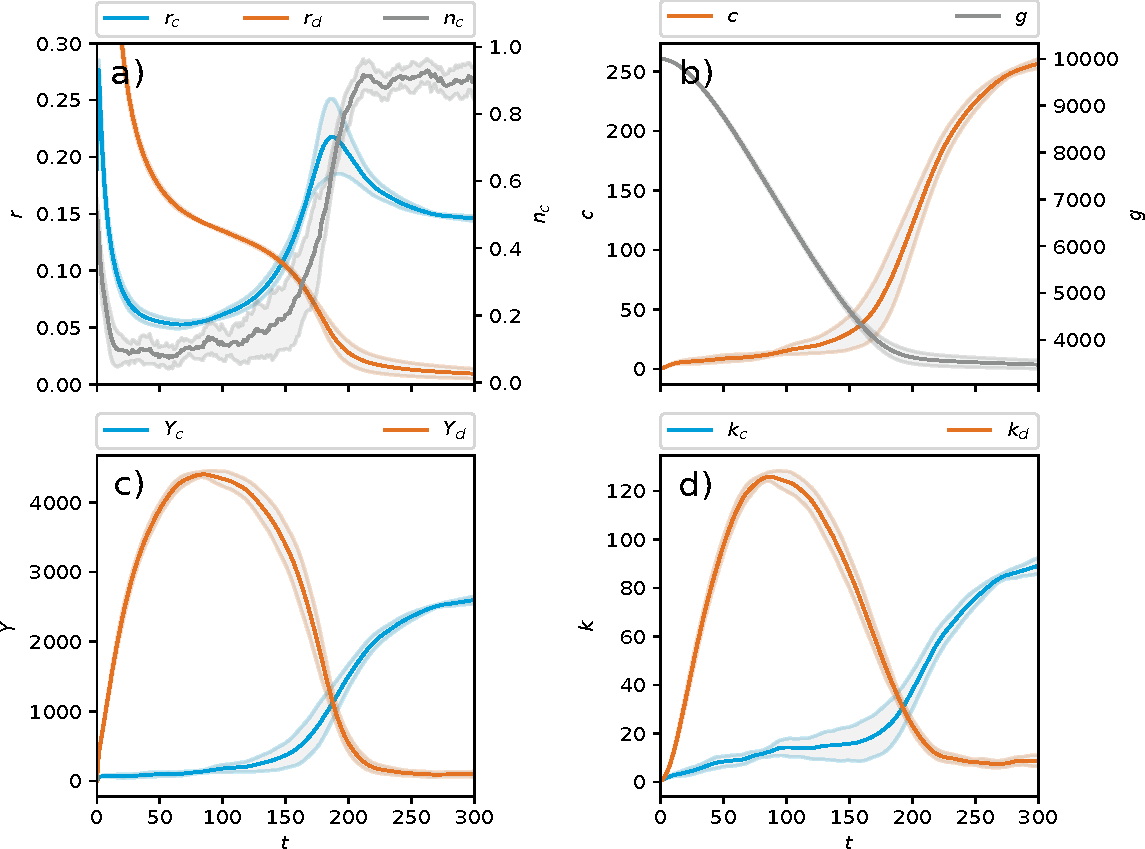
\includegraphics[width=.9\linewidth]{figures/example_trajectory.pdf}
  \caption{\textbf{Example trajectory of the ABM.} Solid lines show mean results from 100 runs of the model in per capita variables. Grey areas around solid lines show their standard deviation. The panels show capital rents in the clean and dirty sector $r_c$ and $r_d$ as well as the fraction of households investing in the clean sector $n_c$ in panel (a), knowledge and resource stock $c$ and $g$ in panel (b), output of clean and dirty sector $Y_c$ and $Y_d$ in panel (c) and per capita capital $k_c$ and $k_d$ in the clean and dirty sector (d).
Initial conditions are $G=G_0$, $C=1$, $K_j^{(i)}=1$ for the economic subsystem. For the investment decision process, the initial opinions of the $N=100$ households are drawn from a uniform distribution. Their initial acquaintance structure is an Erd\H{o}s-Renyi random graph with mean degree k=10.}
\label{fig:example_trajectory}
\end{figure}

Figure \ref{fig:example_trajectory} displays an exemplary trajectory of our model calculated as the mean of 100 simulation runs.
The simulation starts with abundant fossil resources $g$ (panel b) and equally low capital stocks in the clean and dirty sector $k_c$ and $k_d$ in panel d). As we show later (see Sec.~\ref{sec:bifurcation-analysis}), the rest of the initial configuration of the model is rather irrelevant for the selected parameter values listed in Tab.~\ref{tab:Parameter_list}, since there is only one stable dynamical equilibrium as long as resource extraction costs are negligibly low.
The low initial capital in combination with a fixed labor supply leads to high capital rents $r_c$ and $r_d$ that decrease over time as the capital stock is build up.
Initially (from $t=0$ to $t=100$), capital productivity is higher in the dirty sector than the clean sector (see panel a) due to low fossil resource extraction costs. %\FMH{This sentence is incomplete (unclear what the information in brackets means).}
%\JJK{slightly reformulated it. Hope it is clearer now.}
Therefore, the majority of households invest in dirty sector leading to a high per household capital stock $k_c$ (panel c) and high production output $Y_d$ (panel d).

Regarding the capital rents, we would expect the system to move towards a dynamic equilibrium in which the capital rent is equal in both sectors, i.e. $r_d = r_c$, if everything else remained constant.
The difference between $r_c$ and $r_d$ in panel a) can be explained by the exploration in investment strategies, which brings the shares of clean and dirty investors closer together. In terms of the depicted variables this means that it brings $n_c$ closer to $0.5$. 
% \FMH{I reformulated the last sentences, because they were difficult to understand, please check! - Checked}

For $t>100$ the fossil resource is gradually depleted leading to significantly increasing resource extraction costs. Consequently, $r_d$ decreases leading to a peak in accumulation of capital in the dirty sector (panel d).
Once the relative capital returns in the clean sector increase, households start to adopt a clean investment strategy visible in an increase in $n_c$ in panel a).
When the fossil resource stock reaches its economically exploitable share at around $t=200$, the overall productivity in the dirty sector reaches zero, leading to full employment of all available labor in the clean sector.
This drives demand for capital up, accelerating the investment change from clean to dirty investment.
As all households except for the share caused by exploration are investing in the clean sector, the system reaches an equilibrium with high capital in the clean sector and low capital in the dirty sector.

Notably, there is an increasing variance in the fraction of households investing in the clean sector before and around the transition, which means that due to the stochasticity of the social learning process the transition happens earlier for some simulation runs than for others. Nevertheless, the inertia of the model resulting from the large accumulated stock of capital that is specific to the dirty sector eventually leads to an almost entire depletion of the fossil resource.

\begin{table}
	\centering
	\begin{tabular}{l|l|l}
		\hline
		$b_c$ & 1. & Total factor productivity in the clean sector \\
		$b_d$ & 4. & Total factor productivity in the dirty sector \\
		$b_R$ & .1 & Initial resource extraction cost \\
		$e$   & 1 & Resource conversion efficiency \\
		$\kappa$   & 0.06 & Capital depreciation rate \\
		$\chi$      & 0.1 & Knowledge depreciation rate \\
		$\gamma$	   & 0.1 & Elasticity of knowledge in the clean sector \\
		$\alpha_c$ & 0.5 & Elasticity of labor in the clean sector \\
		$\alpha_d$ & 0.5 & Elasticity of labor in the dirty sector \\
		$\beta_c$ & 0.5 & Elasticity of capital in the clean sector \\
		$\beta_d$ & 0.5 & Elasticity of capital in the dirty sector \\
		$\varphi$ & 0.5 & Fraction of rewiring events in opinion formation \\
		$1/\tau$ & 1. & Rate of opinion formation events \\ 
		$\varepsilon$ & 0.05 & Fraction of noise events in opinion formation \\ 
        $G_0$ & 1000000 & Initial resource stock \\
        $L$ & 100 & Total labor \\ 
        \hline
	\end{tabular}
	\caption{List of model parameters with their default values}
	\label{tab:Parameter_list}
\end{table}

\section{Approximate Analytical Solution}
\label{sec:Approximation}

Structurally, the model described in Section \ref{sec:Model_Description} consists of a set of coupled ordinary differential equations \cref{eq:learning_by_doing,eq:resource_depletion,eq:clean_investment,eq:dirty_investment} with algebraic constraints \cref{eq:efficient_dirty_resources,eq:equilibrium_wage,eq:population,eq:clean_capital_rent,eq:dirty_capital_rent} for the economic production process and a stochastic adaptive network process for the social learning component. The state space of this combined process consists of two degrees of freedom of the knowledge stock and the geological resource stock as well as $2N$ degrees of freedom for the capital holdings of the set of all individual households plus the configuration space of the adaptive network process of the social learning component. We denote the variables of this process by capital letters ($C, G, K_j^{(i)}\dots$).
To find an analytic description of the model, we approximate it via a Pair Based Proxy (PBP) process, a stochastic process in terms of aggregated quantities, thereby drastically reducing the dimensionality of the phase space. We denote the variables of this process with capital letter with bars or tildes ($\bar{X}, \bar{Y}, \bar{Z}, \bar{K}_l^{(k)}\dots$).

The derivation of this approximate process is done in three steps: First, we solve the algebraic constraints to the economic production process given by market clearing in the labor market and efficient production in the dirty sector - loosely following \cite{Nitzbon2017}. Second we use a pair approximation to describe the complex adaptive network process of social learning in terms of aggregated variables, similar to \cite{Rogers2012}. Third, we use a moment closure-like method to approximate higher moments of the distribution of the capital holdings of the heterogeneous households by quantities related to the first moments of their distribution.

Finally, we take the limit of infinitely many households (large system- or thermodynamic limit) to obtain a deterministic description of the system.

\subsection{Algebraic Constraints}
%\JJK{Most of this subsection could move to supplementary material to be replaced by a verbal explanation, depending on the journal requirements}
I use the same solution for the algebraic constraints that arise from assumptions about labor and capital markets as in \ref{sec:algebraic_constraints}

\subsection{Pair Approximation}
\label{sec:pair_approximation}
To derive a macroscopic approximation of the social learning process, we make use of a Pair based proxy (PBP) process that is derived via pair approximation from the adaptive network process. This proxy process is not equivalent but sufficiently close to the microscopic process approximating it in terms of aggregated quantities by making certain assumptions about the properties of their microscopic structure. The aggregated quantities of interest are: the number of households investing in clean capital $N^{(c)}$, the number of households investing in dirty capital $N^{(d)}$, the number of links between agents of the same group $[cc]$ and $[dd]$ as well as between the two groups $[cd]$. Since the total number of households $N$ and links $M$ are fixed, these five variables reduce to three degrees of freedom, which we parameterize as follows:

\begin{equation}
	\bar{X} = N^{(c)} - N^{(d)}, \quad \bar{Y} = [cc] - [dd], \quad \bar{Z} = [cd].
	\label{eq:opinion_formation_macro_variables}
\end{equation}

These three degrees of freedom span the reduced state space of the social process $\mathbf{\bar{S}} = (\bar{X}, \bar{Y}, \bar{Z})^T$. The investment decision making process can then be described in terms of jump lengths $\Delta \mathbf{\bar{S}}_j$ and jump rates $W(\mathbf{\bar{S}},\mathbf{\bar{S}} + \Delta \mathbf{\bar{S}}_j)$ in this state space for the different events $j$ in the set $\Omega$ of all possible events.
The derivation of these is illustrated by the example of a clean household imitating a dirty household: The approximate rate of this event is given by
\begin{equation}
	W_{c \rightarrow d} = \frac{N}{\tau} (1-\varepsilon) (1 - \varphi) \frac{N^{(c)}}{N}\frac{[cd]}{[cd] + 2 [cc]}p_{cd}.
	\label{eq:cdswitchingprob}
\end{equation}
In some more detail this results from
\begin{itemize}
	\item $N/\tau$ the rate of social update events i.e. the rate of events per household times the number of households,
	\item $(1-\varepsilon)$ the probability of the event not being a noise event,
	\item $(1-\varphi)$ the probability of imitation events (versus network adaptation events),
	\item $N^{(c)}/N$ the probability of the active households to invest in clean capital,
	\item $[cd]/(2[cc] + [cd])$ the approximate probability of interaction with a household investing in dirty capital. Here, we approximate the distribution of dirty neighbors among clean households with its moment i.e. we act as if links between clean and dirty households were evenly distributed among all households. 
	\item $p_{cd}$ is the expected value of the probability of the active households imitating its neighbor depending on the difference in consumption between households investing in clean and dirty capital as given in equation \eqref{eq:imitation_probability}. The expression is derived in detail as part of the moment closure in subsection \ref{moment_closure}.
\end{itemize}
The corresponding change in the state space variables is a little more tricky. Since the event is a clean household imitating a dirty household, we already know about one of the neighbors of the household. Then the state of the remaining neighbors is approximated by drawing $k^{c} - 1$ times from the distribution of neighbors that is, as before, approximated by an even distribution of edges between same and different households among all households again approximating the respective full distributions with their first moments. Thus the probability for a neighbor to be dirty $p^{(d)}$ or clean $p^{(c)}$ reads:
\begin{equation}
	p^{(c)} = \frac{2 [cc]}{2[cc] + [cd]}; \qquad p^{(d)} = \frac{[cd]}{2[cc] + [cd]}.
\label{eq:neighbordist}
\end{equation}
where $k^{(c)}$ is the mean degree, e.g. the mean number of neighbors of a clean household in the network.

This results in $n^{(c)}$ additional clean neighbors and $n^{(d)}$ additional dirty neighbors. 
\begin{equation}
	n^{(c)} = (1-1/k^{(c)})\frac{2[cc]}{N^{(c)}}; \quad n^{(d)} = (1-1/k^{(c)})\frac{[cd]}{N^{(c)}}.
	\label{eq:additional_neighbors}
\end{equation}

With the results from \eqref{eq:additional_neighbors} the changes in the expected values of the state space variables can be approximated as follows:
\begin{align}
	\Delta N^{(c)} &= -1 \nonumber \\
	\Delta N^{(d)} &= 1 \nonumber \\
	\Delta [cc] & \approx \left( 1 - \frac{1}{k^{(c)}} \right)\frac{2[cc]}{N^{(c)}} \nonumber \\
	\Delta [dd] & \approx \left( 1 - \frac{1}{k^{(c)}} \right)\frac{[cd]}{N^{(c)}} \nonumber \\
	\Delta [cd] & \approx -1 + \left( 1 - \frac{1}{k^{(c)}} \right)\frac{2[cc] - [cd]}{N^{(c)}} \nonumber
\end{align}
and, summing up, the change in the state vector is approximately given by:
\begin{equation}
	\Delta \mathbf{\bar{S}}_{c \rightarrow d} \approx \colvec{3}{-2}{-k^{(c)}}{-1 +  \left( 1 - \frac{1}{k^{(c)}} \right)\frac{2[cc] - [cd]}{N^{(c)}} }.
	\label{cdstatespacechange}
\end{equation}

In terms of the jump lengths $\Delta \mathbf{\bar{S}}$ and the rates $W$, the dynamics of the PBP can be written as a master equation for the probability distribution $P$ on the state space of $\mathbf{\bar{S}}$:

\begin{align}
	\frac{{\partial} P(\mathbf{\bar{S}}, t)}{\partial t} = \sum_{j \in \Omega} &P(\mathbf{\bar{S}} - \Delta \mathbf{\bar{S}}_j, t) W(\mathbf{\bar{S}} - \Delta \mathbf{\bar{S}}_j,\mathbf{\bar{S}}) \nonumber \\
	&- P(\mathbf{\bar{S}}, t) W(\mathbf{\bar{S}},\mathbf{\bar{S}} + \Delta \mathbf{\bar{S}}_j) \label{eq:PBP}
\end{align}

\subsection{Moment Closure}
\label{moment_closure}

To describe the capital structure in the model, we use the cohort of $N^{(c)}$ households investing in clean and the cohort of $N^{(d)}$ households investing in dirty capital and look at the aggregates of their respective capital holdings:
\begin{align}
	\bar{K}_l^{(k)} = \sum_{i}^{N} \delta_{o_ik} K_l^{(i)}%, \qquad \lim_{N \rightarrow \infty} \bar{K}_{l}^{(k)} = \braket{K_l^{(i)}}{o_i = k} = \mu_l^{(k)}
	\label{eq:moments_definition}
\end{align}
Here, the upper index in $\bar{K}_l^{(k)}$ indicates the shared investment decision of the cohort of households as opposed to the index of the individual household before. The lower index still denotes the capital type. $\delta_{o_ik}$ is the Kronecker Delta.

Later, we use the fact that in the limit of $N \rightarrow \infty$ these aggregates should converge their expected values, e.g. the first moments of their distribution with probability one.
The time derivative of the aggregates defined in \eqref{eq:moments_definition} is given by the deterministic process of capital accumulation \eqref{eq:clean_capital_accumulation} and \eqref{eq:dirty_capital_accumulation} as well as terms resulting from the stochastic process of agents switching their saving decisions. 
\begin{equation}
      \begin{aligned}
          \dot{\bar{K}}_c^{(c)} =&  \\
          \dot{\bar{K}}_d^{(c)} =&  \\
          \dot{\bar{K}}_c^{(d)} =&  \\
          \dot{\bar{K}}_d^{(d)} =& 
      \end{aligned}
  \underbrace{ 
      \begin{aligned}
      &(sr_c - \alpha)\bar{K}_c^{(c)} + s r_d \bar{K}_d^{(c)} + s w \bar{L} \\
      &- \alpha\bar{K}_d^{(c)} \\
      &- \alpha\bar{K}_c^{(d)} \\
      &sr_c \bar{K}_c^{(d)} + (s r_d - \alpha)\bar{K}_d^{(d)} + s w \bar{L}
      \end{aligned}
  }_{\textstyle D^{(i)}_{l} } \quad + \mathrm{switching\ terms} \label{eq:sterm0}
\end{equation}
The switching terms for $\bar{K}_c^{(c)}$ result from agents changing their saving decision, thereby moving their capital endowments from the aggregate capital of the cohort of clean investors to the aggregate of the cohort of dirty investors and vice versa. We assume that each household switching to the other cohort is endowed with the mean capital of the cohort and that their capital endowment is independent of the probability of switching such that we can describe the switching terms as a product of both factors. Then, we can write down the changes in capital stocks explicitly including the switching terms as a simple stochastic differential equation:
\begin{equation}
	{\mathrm d}\bar{K}_{l}^{(k)} = D^{(i)}_{l} {\mathrm d}t + \underbrace{\frac{\bar{K}_l^{(j)}}{N^{(j)}} {\mathrm d} N^{j \rightarrow k} -  \frac{\bar{K}_l^{(k)}}{N^{(k)}} {\mathrm d} N^{k \rightarrow j} }_{\text{switching terms}}.
	\label{eq:aggregated_capital_time_derivative}
\end{equation}
where the first term of the right hand side refers to the change in aggregates without switching, as given by the equations of capital accumulation \eqref{eq:sterm0} and the following terms denote the influx and outflux of capital from the aggregate due to households changing their savings decisions.
${\mathrm d} N^{j \rightarrow k}$ denotes the process of a household switching from one opinion to another according to the rules outlined in \ref{sec:investment_decision_making_descr.}. In line with the pair approximation described in \ref{sec:pair_approximation} we approximate them as
\begin{equation}
{\mathrm d} N^{j \rightarrow k} = \sum_{l \in \Omega_{j \rightarrow k}}W_l {\mathrm d}t
\end{equation}
where $\Omega_{j \rightarrow k}$ denotes the set of all events that result in a household changing from cohort $j$ to cohort $k$ and $W_l$ is the rate of the respective event analogously to \eqref{eq:cdswitchingprob}.
%are given by the sum over the rates $W_{i \rightarrow j}$ as illustrated in eq. \eqref{cdswitchingprob} for all types of events that change the number of households investing in the given type of capital.

The imitation probability $p_{cd}$ in eq. \eqref{eq:cdswitchingprob} is approximated as the expected value of eq. \eqref{eq:imitation_probability} when drawing a pair of neighboring households $i$, $j$ as specified. To calculate the expected value, we perform a Taylor expansion in terms of the consumption of the two interacting households $F^{(c)}$ and $F^{(d)}$ around some fixed values $F^{(c)*}$ and $F^{(d)*}$ up to linear order. To maintain the symmetry of the imitation probabilities with respect to the household incomes, we change variables to $\Delta F = F^{(c)} - F^{(d)}$ and $F = F^{(c)} + F^{(d)}$ and expand around $\Delta F = 0, F = F_0$, where $F_0$ is yet to be fixed to a value. In linear order this results in:
\begin{align}
	p_{cd} &= \frac{1}{2} - \frac{a}{4 F_0} \Delta F, \label{eq:approx_p_cd}\\
	p_{dc} &= \frac{1}{2} + \frac{a}{4 F_0} \Delta F. \label{eq:approx_p_dc}
\end{align}

To make the approximation work in the biggest part of the systems state space, we set the reference point $F_0$ to be the middle of the sum of the estimated upper and lower bounds for the attainable income of households investing in the clean, resp. dirty sector. The minimum attainable income is assumed to be zero. The maximum attainable income for a household investing in the clean sector is assumed to be reached in equilibrium given all other households also invest in the clean sector e.g. we calculate $F^{(c)*}$ as half of an average household income at the steady state of $\dot{K}_c = s b_c L^\alpha K_c^{\beta_c} C^\gamma - \delta K_c$ and $\dot{C} = b_c L^\alpha K_c^{\beta_c} C^\gamma - \delta C$:
\begin{equation}
	C^* = \left( \frac{b_c L^\alpha s^{\beta_c}}{\delta}\right)^{\frac{1}{1-\beta_c-\gamma}}, \quad K_c^* = \left( \frac{b_c L^\alpha s^{1-\gamma}}{\delta}\right)^{\frac{1}{1-\beta_c-\gamma}}.
	\label{eq:clean_steady_state}
\end{equation}
Equivalently, we calculate $F^{(d)*}$ as half of an average household income at the steady state of $ \dot{K}_d = s \left(1 - \frac{b_R}{e} \right) b_d K_d^{\beta_d} P^{\alpha} - \delta K_d $:
\begin{equation}
	K_d^* = \left( \frac{s b_d L^\alpha}{\delta} \left(1 - \frac{b_R}{e} \right)\right)^{\left(\frac{1}{1 - \beta_d} \right)}.
	\label{eq:dirty_steady_state}
\end{equation}
With these results, using the fact, that we set $\beta_c = \beta_d = \alpha = 1/2$ the reference point $F_0$ is
\begin{align}
	F_0 &= \frac{1}{2}\left(F^{(c)*} + F^{(d)*}  \right) \nonumber \\
	&= \frac{1-s}{2N}\left(r_c^* K_c^* + w L + r_d^* K_d^* + w L\right) \label{eq:inc_2}\\
	%&= \frac{1}{2N}\left( Y_c^* + \left( 1 - \frac{b_R}{e} \right) Y_d^* \right) \\
	&= \frac{1-s}{2N}\left( \left( \frac{s b_c L^{\alpha}}{\delta^{\beta_c + \gamma}} \right)^{\frac{1}{1-\beta_c - \gamma}} + \frac{s}{\delta}\left( \left( 1 - \frac{b_R}{e} \right) b_d L^{\alpha} \right)^2 \right)
\end{align}
where $r_c^*$ and $r_d^*$ in \eqref{eq:inc_2} are the capital return rates \cref{eq:clean_capital_rent,eq:dirty_capital_rent} in the respective equilibria \cref{eq:clean_steady_state,eq:dirty_steady_state}.

Given this linear approximation of the imitation probabilities, we approximate $F_c$ and $F_d$ as the household income of the average household investing in clean and dirty capital using the aggregated variables as introduced in \eqref{eq:moments_definition} which in the large system limit is equivalent to taking the expected value over all households in the respective cohorts:

\begin{align}
	p_{cd} = \frac{1}{2} - \frac{a}{4 F_0} &\left(r_c\left( \bar{K}_c^{(c)} - \bar{K}_c^{(d)} \right) \right. \nonumber \\ 
	& \left. + r_d\left( \bar{K}_d^{(c)} - \bar{K}_d^{(d)} \right) + w\frac{L}{N}\left( N^{(c)} - N^{(d)} \right) \right) \label{eq:approx_p_cd_final}\\
	p_{dc} = \frac{1}{2} + \frac{a}{4 F_0} &\left(r_c\left( \bar{K}_c^{(c)} - \bar{K}_c^{(d)} \right) \right. \nonumber \\ 
	& \left. + r_d\left( \bar{K}_d^{(c)} - \bar{K}_d^{(d)} \right) + w\frac{L}{N}\left( N^{(c)} - N^{(d)} \right) \right)  \label{eq:approx_p_dc_final}
\end{align}
With this approximation, we have now reached an approximate description of the microscopic dynamics in terms of stochastic differential equations for the aggregate variables.
\subsection{Large System Limit}
\label{sec:large_system_limit}
The description of the model in terms of equations \eqref{eq:PBP} and \eqref{eq:sterm0} pose a significant reduction of complexity, yet it is still a description in terms of a stochastic process rather than in terms of ordinary differential equations, as typically used in macroeconomic models. To derive ordinary differential equations, we do an expansion in terms of system size, which in our case is given by the number of households $N$.
Therefore, following \citet[p. 244]{VanKampen1992}, we introduce the rescaled variables
\begin{equation}
	x = \frac{X}{N}, \quad y = \frac{Y}{M}, \quad z = \frac{Z}{M}, \quad k = \frac{2M}{N}.
	\label{eq:rescalled_pbp_variables}
\end{equation}
and expand the master equation \eqref{eq:PBP} that describes the social learning process in terms of a small parameter $N^{-1}$. In the leading order, the time development of the rescaled state vector $\mathbf{s} = (x, y, z)$ is given by 
\begin{equation}
	\frac{\mathrm{d}}{\mathrm{d}t}\mathbf{s} = \alpha_{1,0}(\mathbf{s})
	\label{macroscopic_equation}
\end{equation}
where $\alpha_{1,0}$ is the first jump moment of $W$. In terms of the rescaled variables $\mathbf{s}$, $\alpha_{1,0}$ is given by
\begin{equation}
	\alpha_{1,0}(\mathbf{s}) = \int \Delta \mathbf{s} W(s, \Delta \mathbf{s}) {\mathrm d} \Delta \mathbf{s},
	\label{eq:jump_moment}
\end{equation}
which in the case of discrete jumps in phase space simplifies to:
\begin{equation}
	\frac{\mathrm{d}}{\mathrm{d}t}\mathbf{s} = \sum_{j \in \Omega}  \Delta \mathbf{s_j} W_j,
	\label{eq:transitions}
\end{equation}
where $\Omega$ is the set of all possible (discrete) events in the opinion formation process.

As for the economic processes, we keep the aggregated quantities $(\bar{K}_i^j, \bar{C}, \bar{G})$ fixed and formally go to a continuum of infinitesimally small households. As people and also households for that matter are finite entities, a continuum of households makes no sense. But practically, this can be understood as an interpretation of the heterogeneous households as a weighted sample of a very large population of heterogeneous individuals and increasing the sample size up until the point where a continuum of households is a sufficiently good approximation of reality in terms of the model. 
The only element in the approximation of the economic model that depends on per household quantities is the imitation probability \eqref{eq:imitation_probability} or rather its approximation \eqref{eq:approx_p_cd} and \eqref{eq:approx_p_dc}. Since we have chosen this to depend on relative differences in income, their dependence on the number of households $N$ cancels out and the limit of $N \rightarrow \infty$ becomes trivial.

It is interesting to note that the freedom to chose equations for economic production that are not scale invariant critically depends on the assumption that household interaction only depends on relative differences. In return one can show that individual interaction that depends on absolute differences only allow for a large system limit if the system is scale invariant in terms of aggregated quantities. Regardless, it would be possible to relax both of these assumptions and to work with the PBP process with the results explicitly depending on the number of households, which in return could lead to interesting finite size effects.


\subsection{Approximation Results}

\begin{figure}[ht!]
\centering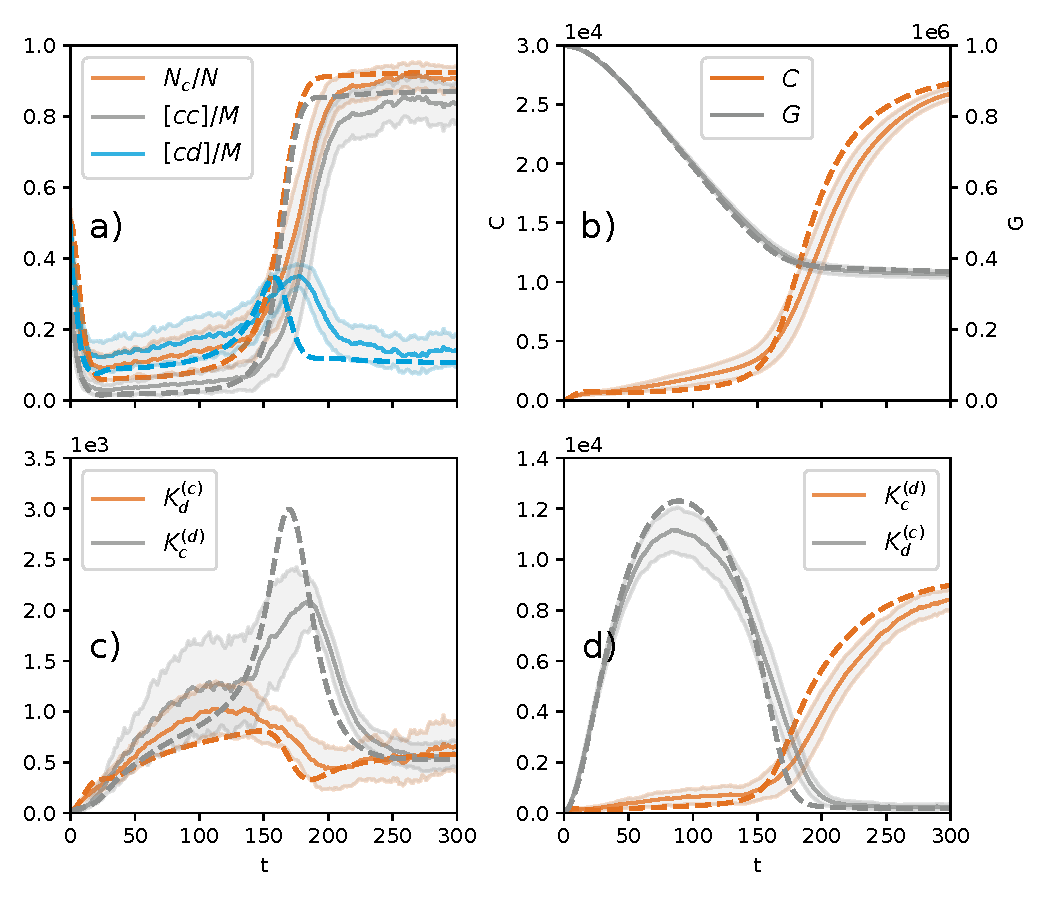
\includegraphics[width=.9\linewidth]{figures/micro_vs_approx_v2_with_annotations.pdf}
\caption{\textbf{Trajectories of dynamic variables from the macro approximation and from measurement in ABM simulations.} The results from ABM simulations (solid lines) are obtained as an ensemble average from 50 runs with standard errors indicated by gray areas. Initial conditions are given by equal shares of the $N=100$ households investing in both sectors and equal endowments in both sectors for all households. The initial acquaintance network amongst the households is an Erd\H{o}s-Renyi random graph with mean degree $k=10$. Other initial conditions are $C_0=0.5$ and $G_0=5 \times 10^5$. All other parameter are given in table \ref{tab:Parameter_list}. The results from the macro approximation (dashed lines of the same colors) are obtained by integration of the ODEs that are obtained from the large system limit with fixed per household quantities. The initial conditions are drawn from the same distribution as previously for the ABM simulations e.g. $N_c$, $[cc]$ and $[cd]$ are calculated from an Erd\H{o}s-Renyi random graph with mean degree $k=10$.}
\label{fig:comparison2}
\end{figure}
%\JK{Maybe better to structure the results as (1), (2), ... and do the same for the full model - then easier to compare}

Comparison of the results of the approximation in fig.~\ref{fig:comparison2} with those of the ABM in fig.~\ref{fig:example_trajectory} shows that the approximation exhibits the same qualitative features as the microscopic model.
This is most visible from panels b) and d) in fig.~\ref{fig:comparison2}. Panel b) displays the same variables as fig.~\ref{fig:example_trajectory}b does for the simulated model in per capita terms.
Panel d) shows capital in both sectors of households that actually invest in these sectors which is almost equivalent to the variables in fig.~\ref{fig:example_trajectory}d as it makes up almost the entirety of these capital stocks. This can be seen in fig. \ref{fig:comparison2}c: It shows capital of households in the sector that they do not currently invest in, which is approximately an order of magnitude smaller (note the different scale of the y-axis in the figure).

Quantitatively, these results show that for the given parameter values the macroscopic approximation is capable of very closely reproducing the states before and after the transition from the dirty to the clean sector, as it lies within the standard error of the ensemble of ABM runs.
The approximation is also reasonably capable to reproduce the timing of the transition even though it estimates it a bit too early. The reason for this might be the slight underestimation of the share of clean investing households, leading to a slight overestimation of the share of dirty capital in the system which is also visible in panel \ref{fig:comparison2}d.

An obvious discrepancy between the micro model and the approximation is the overestimation of dirty capital of clean investors ($K_d^{(c)}$) in the transition phase $t\approx 150$ to $t \approx 200$. This can be explained by the inequality in capital holdings amongst households: In the approximation, all households investing in dirty or clean capital are assumed to have the same income respectively. Therefore, the probability to change their investment behavior will change for all of them at once during the transition phase leading to a rapid shift of dirty investors changing to invest in clean capital but taking their dirty capital endowments with them (hence the sharp peak in dirty capital of clean investors during the transition phase, see fig.  \ref{fig:comparison2}c dashed grey line).

In the micro model, households changing from a dirty to a clean investment strategy take their -- presumably high -- endowments in dirty capital with them. Therefore, the endowments in dirty capital of households investing in the clean sector are relatively wide spread (see grey area around solid grey line in fig. \ref{fig:comparison2}c). 
This also has effects on the estimated timing of the transition. In the micro model, income of households is heterogeneous. Therefore, for each of them the probability to change their investment behavior changes at different points in time, i.e. poorer households are likely to switch earlier during the transition than richer households. Together this leads to a slower, more spread out transition dynamic resulting in a flatter peak in the dirty capital endowments of clean investing households.

Another effect at play during the transition is related to the assumptions in equations \ref{eq:neighbordist} and \ref{eq:additional_neighbors}. Namely, that all households that invest in the same type of capital have the same distribution of clean and dirty neighbors.

However, during a transition these assumptions that are essential to the pair approximation may well be wrong. E.g. a household that has only recently changed its state has a neighborhood that is atypical for its group and adapts only slowly. Consequently, when many changes in the state of the system happen in a short time, a significant proportion of the population is not well described by the approximation.

In the previous section we derived a set of ordinary differential equations describing the stochastic dynamics of an agent based model in terms of aggregated variables in the large system limit. We intend this derivation to be a prototypical example for a macroeconomic model with true microfoundations based on heterogeneous agents, given their microscopic interactions are of similar complexity. As such, it might also serve as a starting point for the application and development of similar models for other kinds of social dynamics. For example, an extension to continuous opinions requiring a Fokker-Planck type description would follow naturally and would grant compatibility to a large body of models for social influence \citep[see ref.][pp. 988 f.]{Mueller-Hansen2017}.

\section{Bifurcation Analysis}
\label{sec:bifurcation-analysis}

The description of the model as a system of ordinary differential equations allows for the analytical analysis of emergent model properties such as multi stability, tipping and phase transitions. 
As a proof of concept application we subsequently show the results of a bifurcation analysis.

\subsection{Methods}
%What is bifurcation analysis?
Bifurcation theory is the analysis of qualitative changes of dynamical systems under parameter variation.
Bifurcation analysis allows identifying parameter ranges of a dynamical system in which multistabilities occur.
For this, families of solutions to a dynamical system are studied with respect to their topology and stability of invariant sets, i.e., regions or points in phase space in which the system stays forever if not perturbed by external influences.
Examples for invariant sets are fixed points, limit cycles, and chaotic attractors or repellers.
A smooth change in a bifurcation parameter can lead to a sudden qualitative change in these properties. For example, fixed points (equilibria) can appear or disappear, they can gain or loose stability and several fixed points can collide and merge.
The parameter value at which such a change occurs is called a critical value or bifurcation point. Bifurcations can be classified according to the changes in dynamical properties of the system.
For a detailed introduction to bifurcation theory, see for example refs. \cite{Strogatz1994,Kuznetsov1998}.
% Methods for Bifurcation Analysis
There are a range of well developed analytical and numerical techniques to study how equilibria change under parameter variation. Because the identification of equilibria in non-linear systems gets easily untractable for analytical methods, a commonly used tool is the numerical continuation method \citep{Allgower2003}.
This is also the case with the system of ordinary differential equations derived in Sec.~\ref{sec:Approximation}. Consequently, we use numerical continuation for our analysis. In particular, we use PyDSTool, a Python package for dynamical systems modeling and analysis, \cite{pydstool,10.1371/journal.pcbi.1002628} building on the AUTO-07p continuation library \cite{Doedel07auto-07p:continuation}.

% Introduce those kinds of bifurcations that we observe in the analysis:
A common bifurcation type that appears in our model is the fold bifurcation that is also known as saddle-node bifurcation. This type is a local bifurcation in which a stable fixed point collides with an unstable one and both disappear. 
%\JK{Normal form ect. necessary here?} It is described by the normal form $\dot{x} = r + x^2$ with bifurcation parameter $r$. The bifurcation point at $r = 0$ divides a regime with two equilibria for $r < 0$ and a regime without any equilibria for $r > 0$.

With a codimension 2 bifurcation analysis, e.g. when varying two different bifurcation parameters at the same time, even richer qualitative changes of the dynamics can be observed. A prevalent example for such a bifurcation is the cusp geometry \citep[][p.\.397]{Kuznetsov1998}. Varying the second bifurcation parameter in this geometry beyond a certain value results in the so-called cusp catastrophe: the multi-stability of the system disappears for all values of the first bifurcation parameter. As we will show in the following, the macro-approximation of our model indeed exhibits a cusp bifurcation. 



\subsection{Discussion of Results}

\begin{figure}[ht!]
\centering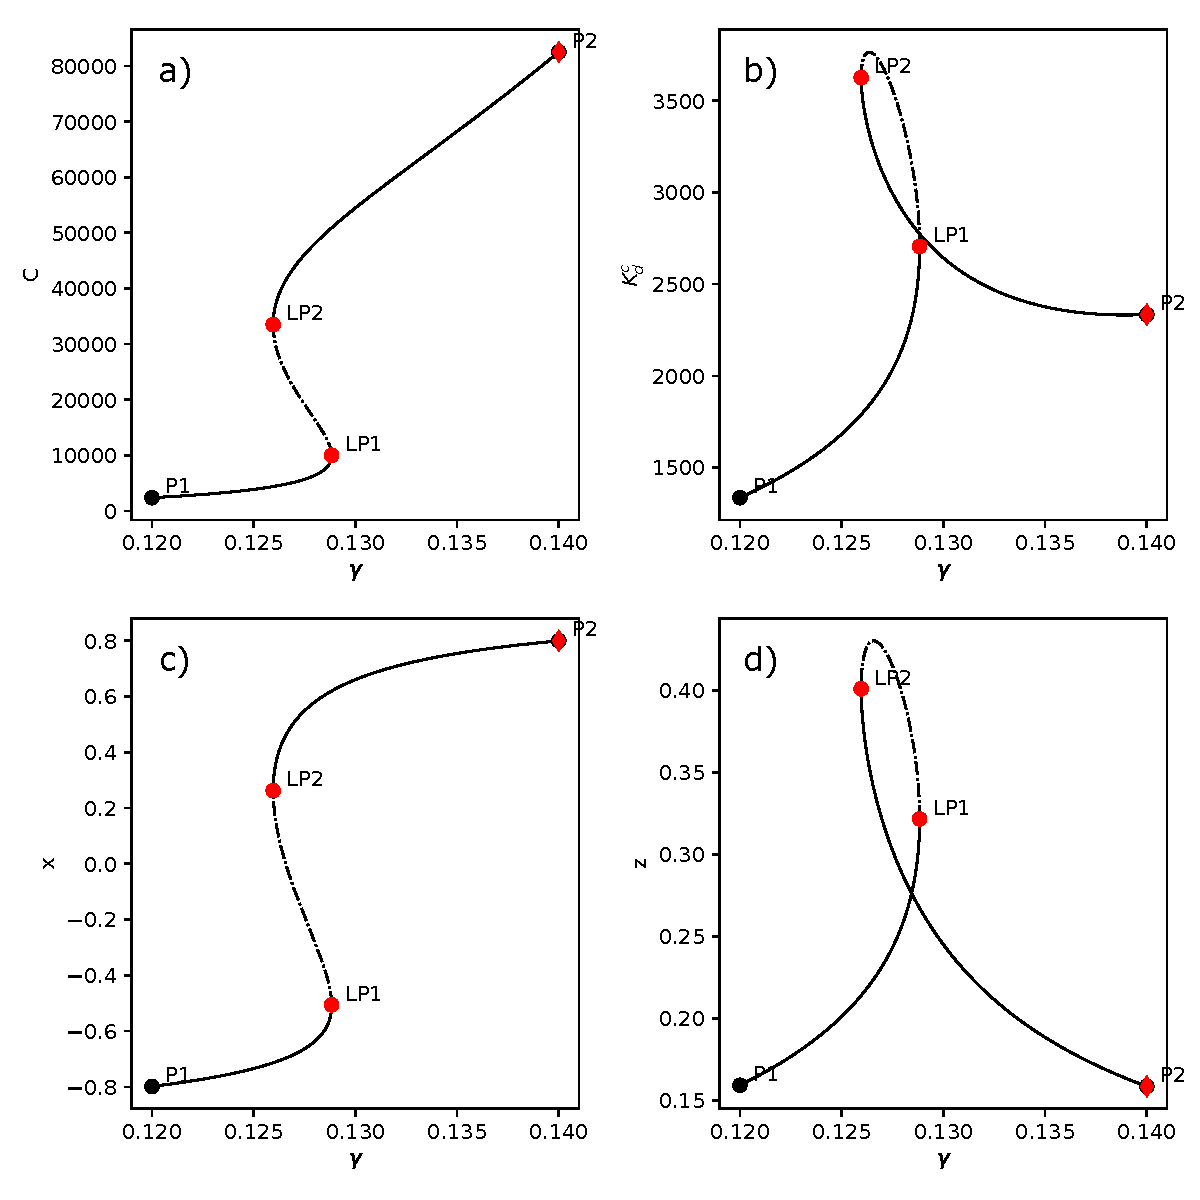
\includegraphics[width=.95\linewidth]{figures/ba_plot.pdf}
\caption{\textbf{Bifurcation diagram:} Continuation of the stationary solution of the macroscopic approximation without resource depletion, e.g. $\dot{G} = 0$ instead of the rate $R$ as given by eq. \eqref{eq:sum_up_resource_depletion}. Bifurcation parameter is $\gamma$, the elasticity of knowledge in the clean sector that also reflects the elasticity of learning by doing of the respective technology. The points labeled P1 and P2 are the beginning and end points of the continuation line, the points labeled LP1 and LP2 are the bifurcation points of two fold bifurcations. The stable unstable manyfold is indicated by a dotted line, the stable manyfold is indicated by solid line. Note that the intersections of the curves in the two right panels do not actually mean that the stationary manifold is not a bijective function of the bifurcation parameter $\gamma$ but rather a result of the projection of the multidimensional manifold onto the two dimensional space.\label{fig:bifurcation_analysis}}
\end{figure}

\begin{figure}[ht!]
\centering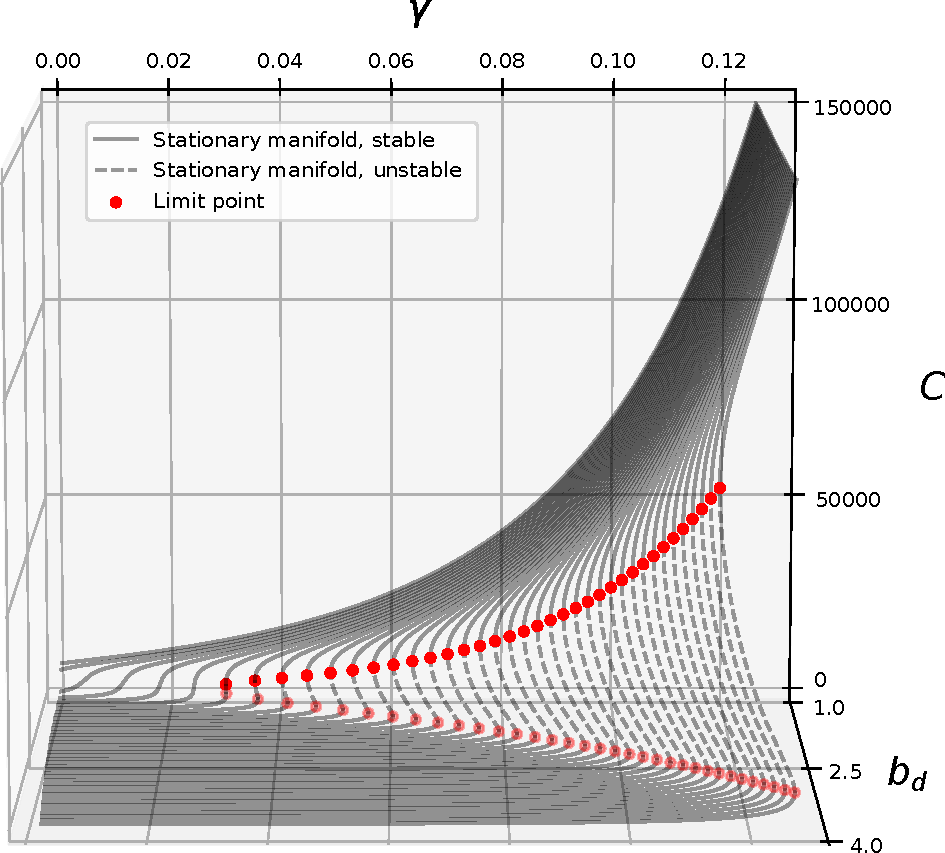
\includegraphics[width=\linewidth]{figures/cusp_better.pdf}
\caption{\textbf{Cusp Bifurcation diagram:}
Stationary manyfold from figure \ref{fig:bifurcation_analysis} panel a) for different values of the total factor productivity on the dirty sector $b_d$. Red dots indicate the limit points of the one dimensional fold bifurcation separating the stable and the unstable parts of the stationary manyfold indicated by a solid and a dashed line respectively. For a critical value of $b_d \approx 1.4$ and $\gamma \approx 0.03034$ the two limit points converge and annihilate each other. This codimension two bifurcation with bifurcation parameters $\gamma$ and $b_d$ is called a cusp catastrophe. In our two-sector economic model, this results in a lock in effect in the dirty sector e.g. below this point, there is a smooth transition of production from the dirty to the clean sector and above this point production in the dirty sector is continued even though production in the clean sector would be more efficient. \label{fig:cusp}}
\end{figure}

A considerable advantage of the description of our model in terms of ordinary differential equations over agent based modeling is the fact that it allows for the usage of established tools for bifurcation analysis.
As a proof of concept, we show some results in figure \ref{fig:bifurcation_analysis}.
Here, we analyze the possible steady states of the system with abundant fossil resources e.g. the possible equilibrium states of the model in the regime before the fossil resource becomes scarce and acts as an external driver on the system pushing it towards clean investment.
Therefore, we set the resource depletion to zero e.g. we keep the resource stock in eq. \eqref{eq:resource_depletion} constant $G(t) \equiv G_0$ such that the resource usage cost in eq. \eqref{eq:resource_cost} still depends on resource use $R$ but is not increased by deceasing resource stock $G$. Thereby, we eliminate the rising resource extraction cost as the constraint in \cref{eq:equilibrium_wage,eq:dirty_capital_rent} that eventually halts production in the dirty sector. 
We chose the learning rate $\gamma$ as bifurcation parameter as we expect it to yield interesting results.
%That is because as an exponent to a dynamical variable it determines its growth pattern leading to subexponential, exponential or superexponential growth for different values \JK{CITATION NEEDED}. \FMH{I would drop the last sentence because this should be only relevant if we would also consider gamma > 1, but this is certainly not a valid parameter value}.
Generally, in nonlinear dynamical systems, exponential factors are expected to have strong influence on dynamical properties. Therefore, changing these factors is expected to lead to bifurcation behavior.
Consequently, in figure \ref{fig:bifurcation_analysis} panel a) and c) we see that for certain learning rates $\gamma$ the macroscopic approximation exhibits a bistable regime limited by two fold bifurcations with bifurcation points indicated by LP1 and LP2.
In this regime both low investment in the clean sector together with hight investment in the dirty sector and low knowledge as well as high investment in the clean sector together with low investment in the dirty sector and high knowledge are stable states of the economic system. This means that in this region economic outcomes are highly path dependent e.g. starting with slightly different knowledge about clean technologies may lead to widely differing adoption levels of the technology in the long run.

Figure \ref{fig:cusp} shows an example of how this bifurcation structure of the dynamical system depends on other parameters. Varying the total factor productivity in the dirty sector $b_d$, the system undergoes a cusp bifurcation. Above a certain value of $b_d$ the system exhibits bi-stability whereas below this value it does not.

%\FMH{Add some words about possible extensions of this analysis?}

Clearly, this choice of bifurcation parameters is only one of many and other choice may very well lead to interesting results. However, we had to limit ourselves to this proof of concept study as an extensive analysis of all possible combinations would be well beyond the scope of this paper.

%\FMH{Do we need this sentence?: Such a configuration would have profound implications on policy design to foster clean technology in order to drive a decarbonization transition in the models production economy.}

Multi-stability of the economy would mean that policies could make use of inherent dynamical properties of the system to reach a desired state or bring the system onto a desired pathway. For example, policy measures such as regulation or taxes can help driving the system into another basin of attraction, i.e. a region of the phase-space in which trajectories approach another equilibrium in the long term. To do so, the system has to cross a separatrix, the boundary between two basins of attraction.
After this boundary is crossed, the policy measure can be discontinued, the system's dynamics guarantee that it reaches the new equilibrium. 
Figure \ref{fig:cusp} shows that such an intervention could be complemented by an additional policy measure, lowering the total factor productivity in the dirty sector, effectively reducing the distance of the stable manyfold from the separatrix and thereby presumably making the first measure less costly.
Another possibility to take advantage of the system's inherent dynamical structure is to use its hysteresis, i.e. to find policy measures that change the first bifurcation parameter $\gamma$ across a bifurcation point or to change the second bifurcation parameter $b_d$ to move the bifurcation point past the current state of the system (or a combination of both) after which the system would fall to the other branch of the stable manyfold. Afterwards, the policy can be discontinued and the system would remain in its new state.
For such considerations, tools from dynamical systems theory and topology can be used to classify the phase-space of the system into regions with respect to the reachability of a desirable state \citep{Heitzig2016,Nitzbon2017}. This allows designing temporary policies that leverage the multi-stability of the socio-economic system.

\section{Conclusion}

% Summary: Method
This paper combines a set of methods to overcome shortcomings of current approaches to base macroeconomic models on microfoundations.
While representative agent approaches are unable to capture dynamics that emerge from structured and local interactions of multiple heterogeneous agents, computational agent-based approaches have the disadvantage that they make tractable model analysis difficult and computationally challenging.
We demonstrated that a combination of approximation techniques allows finding a macro description of a multi-agent system in which heterogeneous agents interact locally on a complex adaptive network as well as via aggregated quantities. 
In contrast to previous analytic work, where the network structure was either static \cite{Lux2016}, restricted to star like clusters \cite{DiGuilmi2012} or approximated by a mean field interaction approach and hence neglected \cite{Aoki1998, Aoki2007, Alfarano2008a, DiGuilmi2008, Chiarella2011a}, we explicitly treat the structure of the adaptive complex interaction network with appropriate approximation methods.

We develop a stylized two-sector investment model, in which investment decisions are driven by a social imitation process, to showcase the three approximations:
First, a pair approximation of networked interactions takes into account the heterogeneity in interaction patterns.
Second, a moment closure approximation makes it possible to deal with heterogeneous attributes that characterize the agents.
Third, the large-system limit abstracts from effects due to finite population size.
It is only possible to take this limit if the model has at least one of the following properties: (i) individual interaction depend only on relative rather than absolute quantities such that the size of households can be decreased while taking the number of households to infinity or (ii) the economic production functions exhibits constant returns to scale such that they scale linearly with the number of households $N$.
The resulting set of ordinary differential equations captures the effect of local interactions at the system level while still allowing for analytical tractability.

% Summary: Results
A comparison between a computational version of the agent-based model and the macro-description reveals that the approximation works well for parameter values distinct from special cases even if only accounting for first moments. Taking more moments into account would increase accuracy but comes at the cost of higher dimensionality and complexity of the macroscopic dynamical system.

% Learnings from model dynamics (topic-wise)
Our model shows that social imitation dynamics add inertia to the investment decisions in the system that cannot be captured by a representative agent approach.
The imitation process results in social learning such that agents tend to direct their investments into the more profitable sector over time.
Because of this, the shift of investments from the dirty (fossil) to the clean (renewable) sector is driven only by economic factors, namely increasing exploration and extraction costs for the fossil energy resource.
Thus, we conclude that neutral imitation of better performing peers is not a feasible mechanism to initiate a bottom-up transformation of the economy. Directed imitation, for example driven by changes in social norms, and supporting policies that make dirty production less profitable are needed to initiate a transformation towards a sustainable economy in the absence of fossil resource shortage.

% Why is analytical description desirable
Finding a system of ordinary differential equations to approximate agent-based models is useful because it makes the analysis of the dynamical properties of the model much easier. One promising application here is bifurcation theory, as illustrated in Sec.~\ref{sec:bifurcation-analysis}.
Furthermore, it opens the possibility to mathematically proof model properties such as the dependency between different parameters and variables in the model.

% Outlook
% discuss further application 
In the context of climate economics and policy, the proposed techniques are especially important because they allow investigating the interplay of learning agents adapting to new policies and effects of shifts in values and preferences. The resulting changes in individual behavior and their impact on macroeconomic dynamics can be studied in a comprehensive modeling framework. 
Large shifts in investments that are required to reach the 2$^\circ$C target are likely to profit from both, policies that rely on price signals, as well as policies that target individual norm change, interaction and behavior not unlike those researched in e.g. the public health context \cite{Zhang2016, Zhang2015, Centola2011}. The presented techniques can help to better understand how such behavioral interventions would impact the macro-level dynamics of the economic system.

% more specific outlook
On this regard, there are several promising avenues to develop the model and approximation techniques further: For example, instead of binary opinions, the social interaction model can use continuous variables to represent gradual opinions, drawing on a variety of models of social influence \citep[see ref.][pp. 988 f.]{Mueller-Hansen2017}.
An approximation of the agent ensemble would then need a Fokker-Planck-type description rather than a master equation.

% economic modifications
Our model could be extended to explicitly include policy instruments such as a carbon tax and explore its impact on the investment decisions of the heterogeneous agent population.
Another promising modification could include consumption decisions into our two-sector model. Consumption decisions are strongly influenced by social norms and interactions \citep{Peattie2010}. Their inclusion could inform the discussion about green consumption as a potential mechanism for a bottom-up transformation towards a more sustainable economy.

\section*{Acknowledgements}
The authors declare that they do not have any conflict of interest. Jakob J. Kolb acknowledges funding by the Foundation of German Industries. Finn M\"{u}ller-Hansen acknowledges funding by the DFG (IRTG 1740/TRP 2011/50151-0).
Numerical analyses were performed on the high-performance computer system of the Potsdam-Institute for Climate Impact Research, supported by the European Regional Development Fund, BMBF, and the Land Brandenburg.
Finally, the authors thank J\"{u}rgen Kurths for extensive comments on the prefinal version of this manuscript.

% \section{Structures from the template to copy paste}

% \begin{itemize}
% \item Bullet point one
% \item Bullet point two
% \end{itemize}

% \begin{enumerate}
% \item Numbered list item one
% \item Numbered list item two
% \end{enumerate}

% \begin{table}[h]
% \centering
% \begin{tabular}{l l l}
% \hline
% \textbf{Treatments} & \textbf{Response 1} & \textbf{Response 2}\\
% \hline
% Treatment 1 & 0.0003262 & 0.562 \\
% Treatment 2 & 0.0015681 & 0.910 \\
% Treatment 3 & 0.0009271 & 0.296 \\
% \hline
% \end{tabular}
% \caption{Table caption}
% \end{table}

% \begin{figure}[h]
% \centering\includegraphics[width=0.4\linewidth]{placeholder}
% \caption{Figure caption}
% \end{figure}

% \begin{equation}
% \label{eq:emc}
% e = mc^2
% \end{equation}

%% The Appendices part is started with the command \appendix;
%% appendix sections are then done as normal sections
%% \appendix

%% \section{}
%% \label{}

%% References
%%
%% Following citation commands can be used in the body text:
%% Usage of \cite is as follows:
%%   \cite{key}          ==>>  [#]
%%   \cite[chap. 2]{key} ==>>  [#, chap. 2]
%%   \citet{key}         ==>>  Author [#]

%% References with bibTeX database:


%        \setpartpreamble{\vspace{1cm} \centering \parbox[l]{9cm}{...}}
%        \part{Applications} \label{part:applications}

	
%	\include{chapter08}
    \appendix
        \addcontentsline{toc}{part}{Appendix}
        \part*{Appendix}
%       \KOMAoptions{paper=a1}
\recalctypearea

Full system of equations resulting from the approximations in section \cref{sec:Approximation}:

\begin{align*}
  \dot{x} = &- \frac{1.0 \epsilon x}{\tau} + \frac{1.0 z \left(\epsilon - 1\right) \left(\phi - 1\right) \left(x - 1\right)}{\tau \left(y - 1\right) \left(e^{\frac{8.0 \left(W_{c} - W_{d}\right)}{W_{c} + W_{d}}} + 1\right)} - \frac{1.0 z \left(\epsilon - 1\right) \left(\phi - 1\right) \left(x + 1\right)}{\tau \left(1 + e^{- \frac{8.0 \left(W_{c} - W_{d}\right)}{W_{c} + W_{d}}}\right) \left(y + 1\right)} \\
%
  \dot{y} = &- \frac{1.0 \epsilon m y}{\tau} + \frac{1.0 m z \left(\epsilon - 1\right) \left(\phi - 1\right)}{\tau \left(e^{\frac{8.0 \left(W_{c} - W_{d}\right)}{W_{c} + W_{d}}} + 1\right)} - \frac{1.0 m z \left(\epsilon - 1\right) \left(\phi - 1\right)}{\tau \left(1 + e^{- \frac{8.0 \left(W_{c} - W_{d}\right)}{W_{c} + W_{d}}}\right)} \\
    & + \frac{\left(x - 1\right) \left(0.25 \epsilon z \left(x - 1\right) - 0.25 \epsilon \left(x + 1\right) \left(y + z - 1\right) + 0.5 \phi z \left(\epsilon - 1\right)\right)}{\tau \left(y - 1\right)} \\
    & + \frac{\left(x + 1\right) \left(0.25 \epsilon z \left(x + 1\right) + 0.25 \epsilon \left(x - 1\right) \left(y - z + 1\right) - 0.5 \phi z \left(\epsilon - 1\right)\right)}{\tau \left(y + 1\right)}\\
%
    \dot{z} = &- \frac{1.0 \epsilon m \left(2 z - 1\right)}{\tau} \\
    &- \frac{0.5 z \left(\epsilon - 1\right) \left(\phi - 1\right) \left(\left(x - 1\right) \left(y - 1\right) - 2 \left(y + 2 z - 1\right) \left(m y - m - 0.5 x + 0.5\right)\right)}{\tau \left(y - 1\right)^{2} \left(e^{\frac{8.0 \left(W_{c}-W_{d}\right)}{W_{c} + W_{d}}} + 1\right)} \\
    & - \frac{0.5 z \left(\epsilon - 1\right) \left(\phi - 1\right) \left(\left(x + 1\right) \left(y + 1\right) - 2 \left(y - 2 z + 1\right) \left(m y + m - 0.5 x - 0.5\right)\right)}{\tau \left(1 + e^{- \frac{8.0 \left(W_{c} - W_{d}\right)}{W_{c} + W_{d}}}\right) \left(y + 1\right)^{2}} \\
    & + \frac{\left(x - 1\right) \left(0.25 \epsilon z \left(x - 1\right) - 0.25 \epsilon \left(x + 1\right) \left(y + z - 1\right) + 0.5 \phi z \left(\epsilon - 1\right)\right)}{\tau \left(y - 1\right)} \\
    & - \frac{\left(x + 1\right) \left(0.25 \epsilon z \left(x + 1\right) + 0.25 \epsilon \left(x - 1\right) \left(y - z + 1\right) - 0.5 \phi z \left(\epsilon - 1\right)\right)}{\tau \left(y + 1\right)}
  \end{align*}
%

\begin{align*}
    \dot{C} = - C \delta + C^{\xi} b_{c} \left(\frac{L \left(C^{\xi} b_{c} \left(K^{(c)}_{c} + K^{(d)}_{c}\right)^{\kappa_{c}}\right)^{\frac{1.0}{1.0 - \pi}}}{\left(b_{d} \left(K^{(c)}_{d} + K^{(d)}_{d}\right)^{\kappa_{d}}\right)^{\frac{1.0}{1.0 - \pi}} \left(1.0 - \frac{G_{0}^{2} b_{R}}{G^{2} e}\right)^{\frac{1.0}{1.0 - \pi}} + \left(C^{\xi} b_{c} \left(K^{(c)}_{c} + K^{(d)}_{c}\right)^{\kappa_{c}}\right)^{\frac{1.0}{1.0 - \pi}}}\right)^{\pi} \left(K^{(c)}_{c} \left(\frac{x}{2} + \frac{1}{2}\right) + K^{(d)}_{c} \left(\frac{1}{2} - \frac{x}{2}\right)\right)^{\kappa_{c}}
\end{align*}
\begin{align*}
    \dot{G} = - \frac{L^{\pi} b_{d}}{e} \left(\frac{\left(b_{d} \left(K^{(c)}_{d} + K^{(d)}_{d}\right)^{\kappa_{d}}\right)^{\frac{1.0}{1.0 - \pi}} \left(1.0 - \frac{G_{0}^{2} b_{R}}{G^{2} e}\right)^{\frac{1.0}{1.0 - \pi}}}{\left(b_{d} \left(K^{(c)}_{d} + K^{(d)}_{d}\right)^{\kappa_{d}}\right)^{\frac{1.0}{1.0 - \pi}} \left(1.0 - \frac{G_{0}^{2} b_{R}}{G^{2} e}\right)^{\frac{1.0}{1.0 - \pi}} + \left(C^{\xi} b_{c} \left(K^{(c)}_{c} + K^{(d)}_{c}\right)^{\kappa_{c}}\right)^{\frac{1.0}{1.0 - \pi}}}\right)^{\pi} \left(K^{(c)}_{d} + K^{(d)}_{d}\right)^{\kappa_{d}}
\end{align*}
  \begin{align*}
    \dot{K}_c^{(c)}=& - \delta K^{(c)}_{c} \\
&+ \frac{K^{(c)}_{c} L^{\pi} \kappa_{c} s \left(C^{\xi} b_{c} \left(K^{(c)}_{c} + K^{(d)}_{c}\right)^{\kappa_{c}}\right)^{\frac{1.0}{1.0 - \pi}} \left(\left(b_{d} \left(K^{(c)}_{d} + K^{(d)}_{d}\right)^{\kappa_{d}}\right)^{\frac{1.0}{1.0 - \pi}} \left(1.0 - \frac{G_{0}^{2} b_{R}}{G^{2} e}\right)^{\frac{1.0}{1.0 - \pi}} + \left(C^{\xi} b_{c} \left(K^{(c)}_{c} + K^{(d)}_{c}\right)^{\kappa_{c}}\right)^{\frac{1.0}{1.0 - \pi}}\right)^{- \pi}}{K^{(c)}_{c} + K^{(d)}_{c}} \\
&+ \frac{K^{(c)}_{d} L^{\pi} \kappa_{d} s \left(b_{d} \left(K^{(c)}_{d} + K^{(d)}_{d}\right)^{\kappa_{d}}\right)^{\frac{1.0}{1.0 - \pi}} \left(1.0 - \frac{G_{0}^{2} b_{R}}{G^{2} e}\right)^{\frac{1.0}{1.0 - \pi}} \left(\left(b_{d} \left(K^{(c)}_{d} + K^{(d)}_{d}\right)^{\kappa_{d}}\right)^{\frac{1.0}{1.0 - \pi}} \left(1.0 - \frac{G_{0}^{2} b_{R}}{G^{2} e}\right)^{\frac{1.0}{1.0 - \pi}} + \left(C^{\xi} b_{c} \left(K^{(c)}_{c} + K^{(d)}_{c}\right)^{\kappa_{c}}\right)^{\frac{1.0}{1.0 - \pi}}\right)^{- \pi}}{K^{(c)}_{d} + K^{(d)}_{d}} \\
&+ L L^{\pi - 1.0} \pi s \left(\left(b_{d} \left(K^{(c)}_{d} + K^{(d)}_{d}\right)^{\kappa_{d}}\right)^{\frac{1.0}{1.0 - \pi}} \left(1.0 - \frac{G_{0}^{2} b_{R}}{G^{2} e}\right)^{\frac{1.0}{1.0 - \pi}} + \left(C^{\xi} b_{c} \left(K^{(c)}_{c} + K^{(d)}_{c}\right)^{\kappa_{c}}\right)^{\frac{1.0}{1.0 - \pi}}\right)^{1.0 - \pi} \\
&- \frac{1.0 K^{(c)}_{c} \left(x + 1\right) \left(0.25 \epsilon \left(1 + e^{- \frac{8.0 \left(W_{c} - W_{d}\right)}{W_{c} + W_{d}}}\right) \left(y + 1\right) + 0.5 z \left(\epsilon - 1\right) \left(\phi - 1\right)\right)}{\tau \left(1 + e^{- \frac{8.0 \left(W_{c} - W_{d}\right)}{W_{c} + W_{d}}}\right) \left(y + 1\right)} \\
&- \frac{1.0 K^{(d)}_{c} \left(x - 1\right) \left(0.25 \epsilon \left(y - 1\right) \left(e^{\frac{8.0 \left(W_{c} - W_{d}\right)}{W_{c} + W_{d}}} + 1\right) - 0.5 z \left(\epsilon - 1\right) \left(\phi - 1\right)\right)}{\tau \left(y - 1\right) \left(e^{\frac{8.0 \left(W_{c} - W_{d}\right)}{W_{c} + W_{d}}} + 1\right)}
%
\end{align*}
\begin{align*}
%
  \dot{K}_d^{(c)}=&- K^{(c)}_{d} \delta - \frac{1.0 K^{(c)}_{d} \left(x + 1\right) \left(0.25 \epsilon \left(1 + e^{- \frac{8.0 \left(W_{c} - W_{d}\right)}{W_{c} + W_{d}}}\right) \left(y + 1\right) + 0.5 z \left(\epsilon - 1\right) \left(\phi - 1\right)\right)}{\tau \left(1 + e^{- \frac{8.0 \left(W_{c} - W_{d}\right)}{W_{c} + W_{d}}}\right) \left(y + 1\right)} \\
&- \frac{1.0 K^{(d)}_{d} \left(x - 1\right) \left(0.25 \epsilon \left(y - 1\right) \left(e^{\frac{8.0 \left(W_{c} - W_{d}\right)}{W_{c} + W_{d}}} + 1\right) - 0.5 z \left(\epsilon - 1\right) \left(\phi - 1\right)\right)}{\tau \left(y - 1\right) \left(e^{\frac{8.0 \left(W_{c} - W_{d}\right)}{W_{c} + W_{d}}} + 1\right)}\\
%
\dot{K}_c^{(d)}=& - K^{(d)}_{c} \delta +\frac{1.0 K^{(c)}_{c} \left(x + 1\right) \left(0.25 \epsilon \left(y + 1\right) \left(e^{\frac{8.0 \left(- W_{c} + W_{d}\right)}{W_{c} + W_{d}}} + 1\right) + 0.5 z \left(\epsilon - 1\right) \left(\phi - 1\right)\right)}{\tau \left(y + 1\right) \left(e^{\frac{8.0 \left(- W_{c} + W_{d}\right)}{W_{c} + W_{d}}} + 1\right)} \\
&+ \frac{1.0 K^{(d)}_{c} \left(x - 1\right) \left(0.25 \epsilon \left(y - 1\right) \left(e^{\frac{8.0 \left(W_{c} - W_{d}\right)}{W_{c} + W_{d}}} + 1\right) - 0.5 z \left(\epsilon - 1\right) \left(\phi - 1\right)\right)}{\tau \left(y - 1\right) \left(e^{\frac{8.0 \left(W_{c} - W_{d}\right)}{W_{c} + W_{d}}} + 1\right)}
\end{align*}
\begin{align*}
  \dot{K}_d^{(d)} =& - \delta K^{(d)}_{d} \\
    &+ \frac{K^{(d)}_{d} L^{\pi} \kappa_{d} s \left(b_{d} \left(K^{(c)}_{d} + K^{(d)}_{d}\right)^{\kappa_{d}}\right)^{\frac{1.0}{1.0 - \pi}} \left(1.0 - \frac{G_{0}^{2} b_{R}}{G^{2} e}\right)^{\frac{1.0}{1.0 - \pi}} \left(\left(b_{d} \left(K^{(c)}_{d} + K^{(d)}_{d}\right)^{\kappa_{d}}\right)^{\frac{1.0}{1.0 - \pi}} \left(1.0 - \frac{G_{0}^{2} b_{R}}{G^{2} e}\right)^{\frac{1.0}{1.0 - \pi}} + \left(C^{\xi} b_{c} \left(K^{(c)}_{c} + K^{(d)}_{c}\right)^{\kappa_{c}}\right)^{\frac{1.0}{1.0 - \pi}}\right)^{- \pi}}{K^{(c)}_{d} + K^{(d)}_{d}} \\
    &+ \frac{K^{(d)}_{c} L^{\pi} \kappa_{c} s \left(C^{\xi} b_{c} \left(K^{(c)}_{c} + K^{(d)}_{c}\right)^{\kappa_{c}}\right)^{\frac{1.0}{1.0 - \pi}} \left(\left(b_{d} \left(K^{(c)}_{d} + K^{(d)}_{d}\right)^{\kappa_{d}}\right)^{\frac{1.0}{1.0 - \pi}} \left(1.0 - \frac{G_{0}^{2} b_{R}}{G^{2} e}\right)^{\frac{1.0}{1.0 - \pi}} + \left(C^{\xi} b_{c} \left(K^{(c)}_{c} + K^{(d)}_{c}\right)^{\kappa_{c}}\right)^{\frac{1.0}{1.0 - \pi}}\right)^{- \pi}}{K^{(c)}_{c} + K^{(d)}_{c}} \\
    &+ L L^{\pi - 1.0} \pi s \left(\left(b_{d} \left(K^{(c)}_{d} + K^{(d)}_{d}\right)^{\kappa_{d}}\right)^{\frac{1.0}{1.0 - \pi}} \left(1.0 - \frac{G_{0}^{2} b_{R}}{G^{2} e}\right)^{\frac{1.0}{1.0 - \pi}} + \left(C^{\xi} b_{c} \left(K^{(c)}_{c} + K^{(d)}_{c}\right)^{\kappa_{c}}\right)^{\frac{1.0}{1.0 - \pi}}\right)^{1.0 - \pi} \\
    &+ \frac{1.0 K^{(c)}_{d} \left(x + 1\right) \left(0.25 \epsilon \left(y + 1\right) \left(e^{\frac{8.0 \left(- W_{c} + W_{d}\right)}{W_{c} + W_{d}}} + 1\right) + 0.5 z \left(\epsilon - 1\right) \left(\phi - 1\right)\right)}{\tau \left(y + 1\right) \left(e^{\frac{8.0 \left(- W_{c} + W_{d}\right)}{W_{c} + W_{d}}} + 1\right)} \\
    &+ \frac{1.0 K^{(d)}_{d} \left(x - 1\right) \left(0.25 \epsilon \left(y - 1\right) \left(e^{\frac{8.0 \left(W_{c} - W_{d}\right)}{W_{c} + W_{d}}} + 1\right) - 0.5 z \left(\epsilon - 1\right) \left(\phi - 1\right)\right)}{\tau \left(y - 1\right) \left(e^{\frac{8.0 \left(W_{c} - W_{d}\right)}{W_{c} + W_{d}}} + 1\right)}
\end{align*}

Where $W_d$ and $W_c$ are given by:
\begin{align*}
%
  W_c =& \frac{K^{c}_{c} L^{\pi} \kappa_{c} \left(C^{\xi} b_{c} \left(K^{c}_{c} + K^{d}_{c}\right)^{\kappa_{c}}\right)^{\frac{1.0}{1.0 - \pi}} \left(C^{\frac{1.0 \xi}{1.0 - \pi}} b_{c}^{\frac{1.0}{1.0 - \pi}} \left(K^{c}_{c} + K^{d}_{c}\right)^{\frac{1.0 \kappa_{c}}{1.0 - \pi}} + \left(b_{d} \left(K^{c}_{d} + K^{d}_{d}\right)^{\kappa_{d}}\right)^{\frac{1.0}{1.0 - \pi}} \left(1.0 - \frac{G_{0}^{2} b_{R}}{G^{2} e}\right)^{\frac{1.0}{1.0 - \pi}}\right)^{- \pi}}{K^{c}_{c} + K^{d}_{c}} \\
  &+ \frac{K^{c}_{d} L^{\pi} \kappa_{d} \left(b_{d} \left(K^{c}_{d} + K^{d}_{d}\right)^{\kappa_{d}}\right)^{\frac{1.0}{1.0 - \pi}} \left(1.0 - \frac{G_{0}^{2} b_{R}}{G^{2} e}\right)^{\frac{1.0}{1.0 - \pi}} \left(C^{\frac{1.0 \xi}{1.0 - \pi}} b_{c}^{\frac{1.0}{1.0 - \pi}} \left(K^{c}_{c} + K^{d}_{c}\right)^{\frac{1.0 \kappa_{c}}{1.0 - \pi}} + \left(b_{d} \left(K^{c}_{d} + K^{d}_{d}\right)^{\kappa_{d}}\right)^{\frac{1.0}{1.0 - \pi}} \left(1.0 - \frac{G_{0}^{2} b_{R}}{G^{2} e}\right)^{\frac{1.0}{1.0 - \pi}}\right)^{- \pi}}{K^{c}_{d} + K^{d}_{d}}, \\
%
  W_d =& \frac{K^{d}_{c} L^{\pi} \kappa_{c} \left(C^{\xi} b_{c} \left(K^{c}_{c} + K^{d}_{c}\right)^{\kappa_{c}}\right)^{\frac{1.0}{1.0 - \pi}} \left(C^{\frac{1.0 \xi}{1.0 - \pi}} b_{c}^{\frac{1.0}{1.0 - \pi}} \left(K^{c}_{c} + K^{d}_{c}\right)^{\frac{1.0 \kappa_{c}}{1.0 - \pi}} + \left(b_{d} \left(K^{c}_{d} + K^{d}_{d}\right)^{\kappa_{d}}\right)^{\frac{1.0}{1.0 - \pi}} \left(1.0 - \frac{G_{0}^{2} b_{R}}{G^{2} e}\right)^{\frac{1.0}{1.0 - \pi}}\right)^{- \pi}}{K^{c}_{c} + K^{d}_{c}}\\
  &+ \frac{K^{d}_{d} L^{\pi} \kappa_{d} \left(b_{d} \left(K^{c}_{d} + K^{d}_{d}\right)^{\kappa_{d}}\right)^{\frac{1.0}{1.0 - \pi}} \left(1.0 - \frac{G_{0}^{2} b_{R}}{G^{2} e}\right)^{\frac{1.0}{1.0 - \pi}} \left(C^{\frac{1.0 \xi}{1.0 - \pi}} b_{c}^{\frac{1.0}{1.0 - \pi}} \left(K^{c}_{c} + K^{d}_{c}\right)^{\frac{1.0 \kappa_{c}}{1.0 - \pi}} + \left(b_{d} \left(K^{c}_{d} + K^{d}_{d}\right)^{\kappa_{d}}\right)^{\frac{1.0}{1.0 - \pi}} \left(1.0 - \frac{G_{0}^{2} b_{R}}{G^{2} e}\right)^{\frac{1.0}{1.0 - \pi}}\right)^{- \pi}}{K^{c}_{d} + K^{d}_{d}}.
\end{align*}

\KOMAoptions{paper=a4}
\recalctypearea


        %\nocite{*}
		% See the documentation or under
		% http://edoc.hu-berlin.de/e_autoren/latex/bedingung.php
		% for the list of the permitted styles.
    \backmatter
    \bibliographystyle{plainnat}
    \bibliography{library.bib}
	%\printbibliography % biblatex bibliography
        %\printindex
        \selectlanguage{ngerman}

% You can change this text, if needed.
\chapter*{Selbst"andigkeitserkl"arung}

Ich erkl"are, dass ich die vorliegende Arbeit selbst"andig und nur unter Verwendung der angegebenen Literatur und Hilfsmittel angefertigt habe.

\vspace{2\baselineskip}
\noindent Potsdam, den \today \hfill\authorfirstname \authorsurname    % Use our template or write your own.
\end{document}
